\documentclass[12pt,onecolumn]{article}
\usepackage[utf8]{inputenc} % UTF8 input encoding
\usepackage[T2A]{fontenc}   % T2A font encoding for Cyrillic script
\usepackage[russian]{babel} % Russian language support
\usepackage{listings}
\usepackage{float}
\usepackage{mathtools}
\everymath{\displaystyle}
\usepackage{listings} 
\usepackage[usenames]{color}
\usepackage{geometry}
\usepackage{verbatim}
\usepackage{tabularray}
\usepackage{color}
\usepackage{hyperref}
\newcommand{\nparagraph}[1]{\paragraph{#1}\mbox{}\\}
\geometry{
  a4paper,
  top=20mm, 
  right=25mm, 
  bottom=20mm, 
  left=20mm
}

\begin{document}
\setcounter{tocdepth}{4}
\begin{center}
    Федеральное государственное автономное образовательное учреждение высшего образования "Национальный Исследовательский Университет ИТМО"\\ 
    Мегафакультет Компьютерных Технологий и Управления\\
    Факультет Программной Инженерии и Компьютерной Техники \\
    
\includegraphics[scale=0.3]{image/itmo.jpg} % нужно закинуть картинку логтипа в папку с отчетом
\end{center}
\vspace{1cm}


\begin{center}
    \textbf{Лабораторная работа 1}\\
    по дисциплине\\
    \textbf{Компьютерные сети}
\end{center}

\vspace{2cm}

\begin{flushright}
  Выполнил Студент  группы P33102\\
  \textbf{Лапин Алексей Александрович}\\
  Преподаватель: \\
  \textbf{Авксентьева Елена Юрьевна}\\
\end{flushright}

\vspace{6cm}
\begin{center}
    г. Санкт-Петербург\\
    2023г.
\end{center}

\newpage
\tableofcontents
\newpage

\section*{Цель работы}\addcontentsline{toc}{section}{Цель работы}
Изучение принципов построения и настройки моделей компьютерных сетей в среде NetEmul.

В процессе выполнения лабораторной работы (ЛР) необходимо:

\begin{enumerate}
    \item построить три простейшие модели компьютерной сети;
    \item выполнить настройку сети, заключающуюся в присвоении IP-адрес интерфейсам сети;
    \item выполнить тестирование разработанных сетей путем проведения экспериментов по передаче данных на основе протокола UDP;
    \item сохранить разработанные модели компьютерных сетей для демонстрации процессов передачи данных при защите лабораторной работы.
\end{enumerate}
\section*{Вариант}

P33102 Лапин Алексей Александрович

Ф = 5, И = 7, О = 13, Н = 2

Исходный адрес: $(192 + 13 + 2).(5+2).(7+2).(5+7) = 207.7.9.12$


\section{Знакомство с NetEmul на примере простейшей сети из двух компьютеров}
\subsection{Построение сети.}
Связал 2 компьютера, назначил им имена для удобства. Сверху добавил их IP и MAC-адреса для наглядности.
\begin{figure}[H]
  \centering
  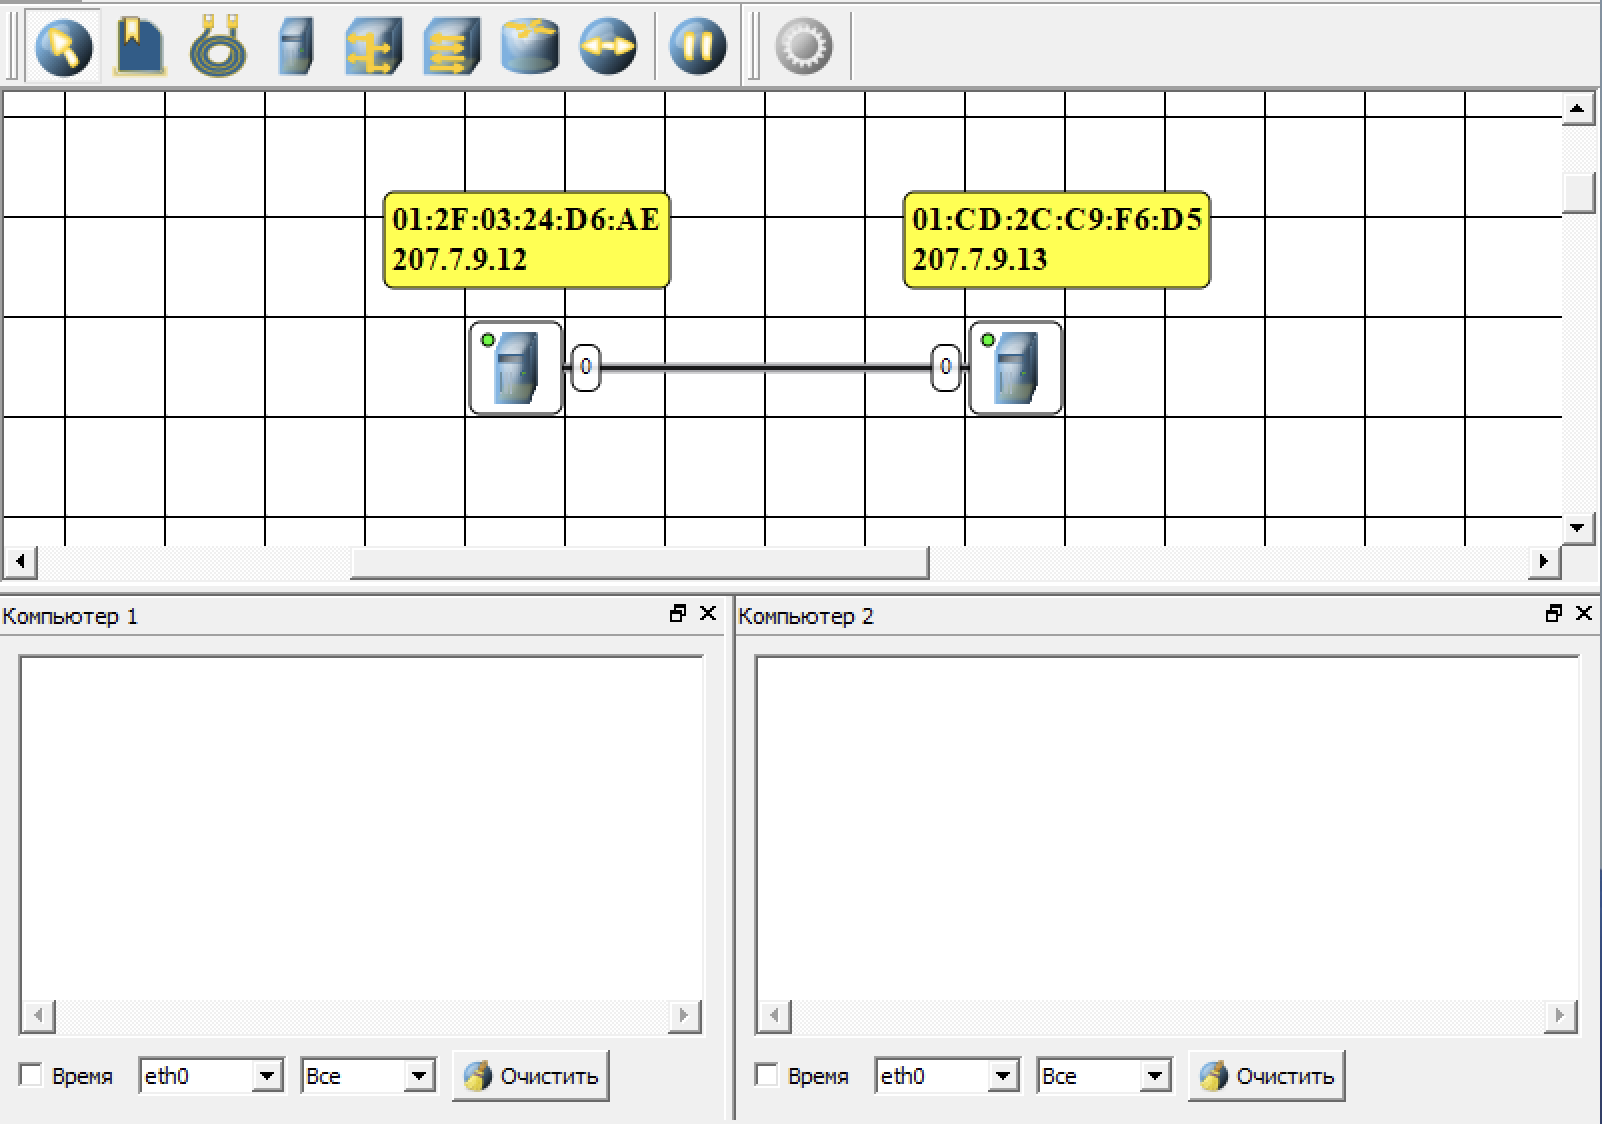
\includegraphics[width=0.8\textwidth]{image/netemul-1-1.png}
  \caption{Журналы устройств с подключением.}
\end{figure}
\begin{figure}[H]
  \centering
  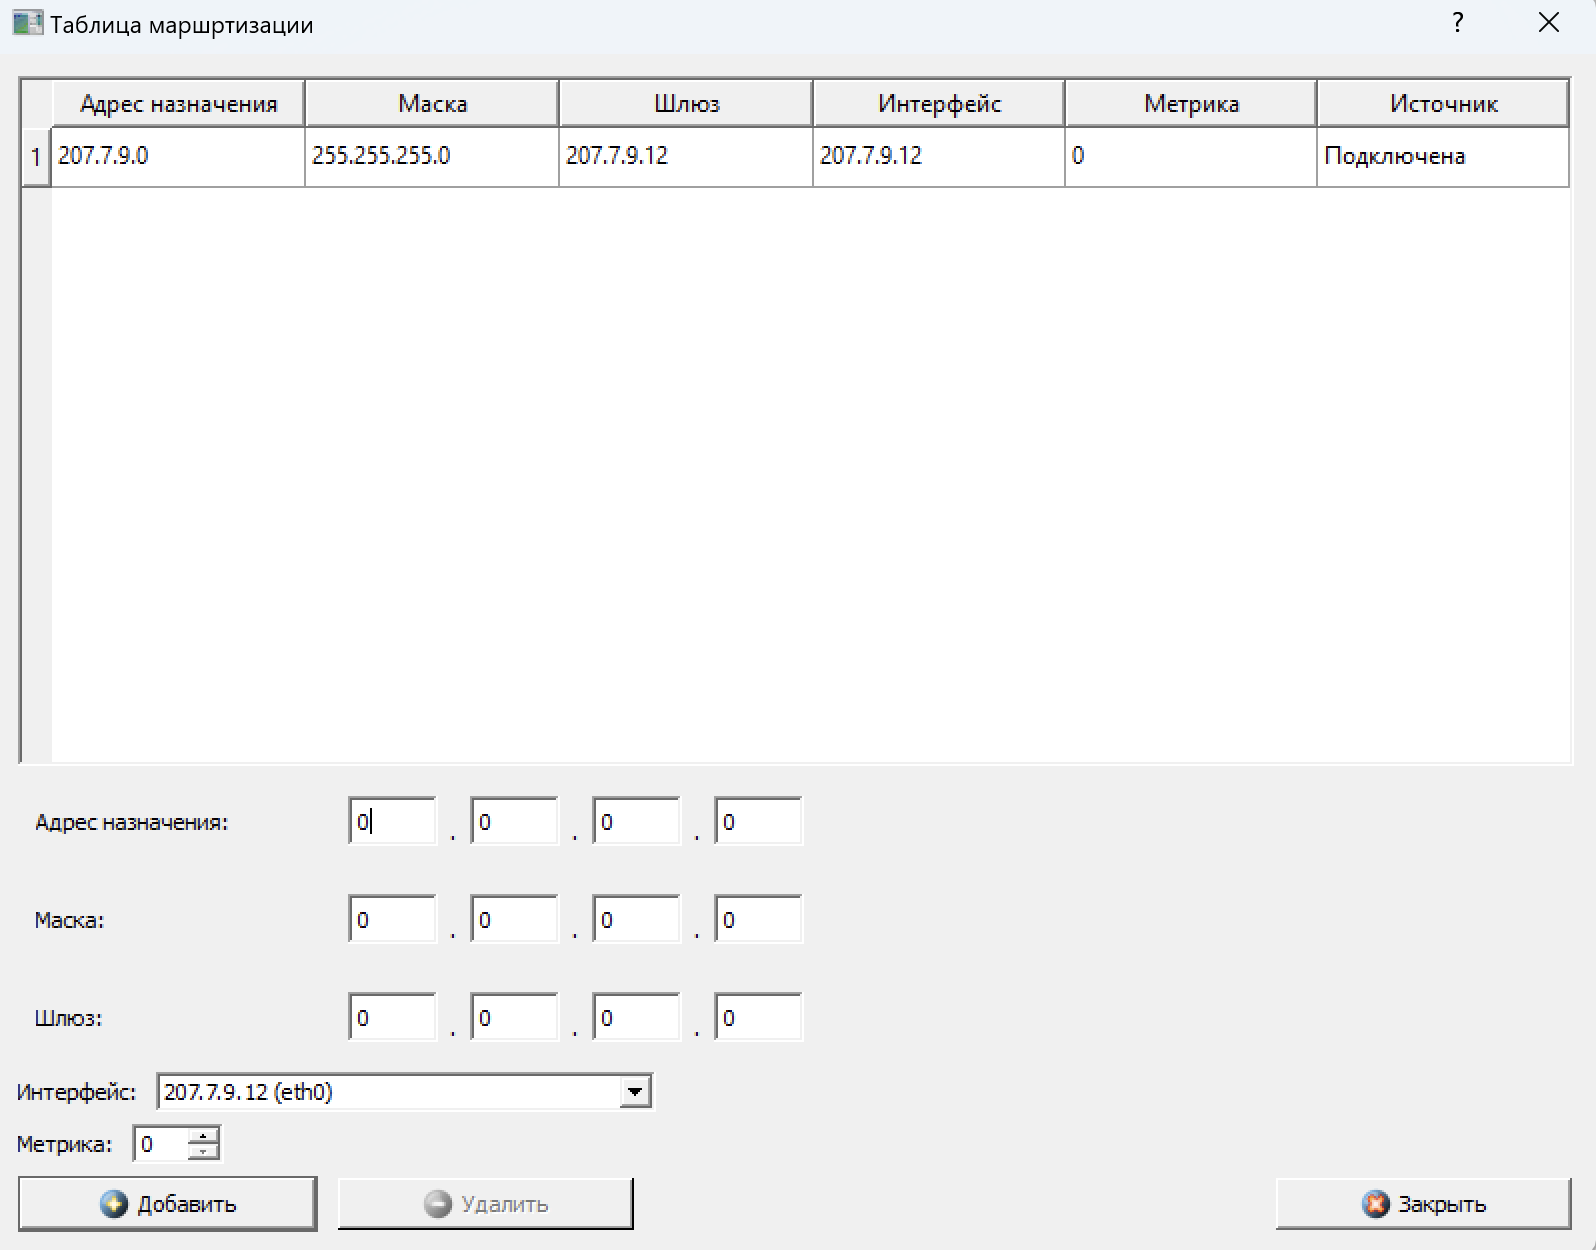
\includegraphics[width=0.8\textwidth]{image/netemul-1-2.png}
  \caption{Таблица маршрутизации.}
\end{figure}
\begin{figure}[H]
  \centering
  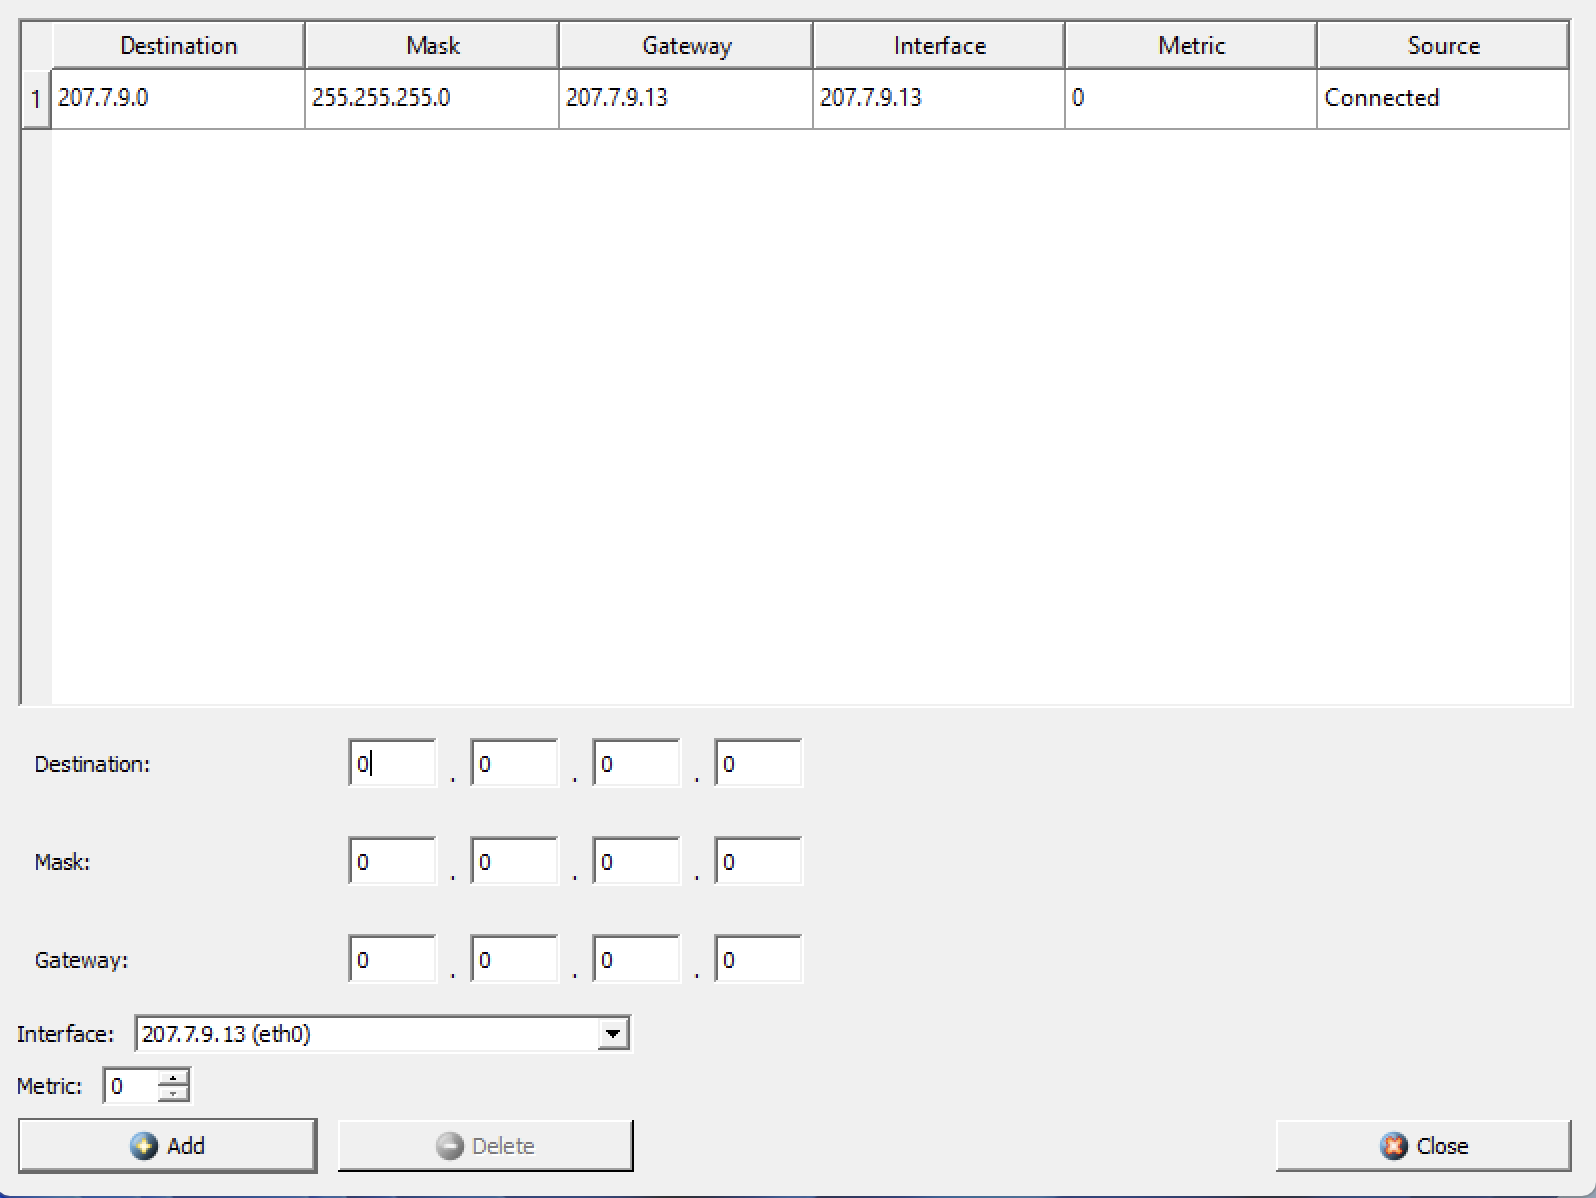
\includegraphics[width=0.8\textwidth]{image/routing-table-2.png}
  \caption{Таблица маршрутизации.}
\end{figure}
\subsubsection{Таблица маршрутизации}
\label{sec:routing}
Таблица маршрутизации — это таблица данных, хранящаяся в маршрутизаторе, в которой перечислены маршруты к определенным сетевым пунктам назначения. Она содержит информацию о топологии сети непосредственно вокруг него.

В простейшем случае таблица состоит из адресов назначения, в соответствии которым ставится адрес следующего соседнего узла нашего маршрутизатора.

В нашем случае таблица маршрутизации состоит из следующих полей:
\begin{enumerate}
  \item Адрес назначения -- адрес подсети, к которой относится маршрут.
  \item Маска -- маска подсети для определения адресов узлов в данной сети.
  \item Адрес и маска подсети вместе задают адреса подсети.
  \item Интерфейс -- адаптор, на который нужно отправлять пакеты к указанной сети. (сетевые карты, обратная петля)
  \item Шлюз -- адрес маршрутизатора, через который нужно отправлять пакеты к указанной сети.
  \item Метрика --  определяет предпочтение для маршрута, когда есть варианты. Строчки с наименьшей метрикой предпочтительны при совпадении диапазонов.
  \item Источник -- источник появления записи в таблице маршрутизации.
\end{enumerate}

Статические маршруты - это записи, сделанные в таблице маршрутизации неавтоматическим способом и являющиеся фиксированными, а не результатом работы протоколов маршрутизации, адаптированных к изменяющимся условиям сети.
\subsubsection{ARP-таблица}
\label{sec:arp}
ARP (Address Resolution Protocol, RFC 826) — протокол для определения соответствия между логическим адресом сетевого уровня (IP) и физическим адресом устройства (MAC).

ARP таблица содержит следующие поля:
\begin{enumerate}
  \item IP-адрес -- адрес сетевого узла в локальной сети.
  \item MAC-адрес --  физический адрес сетевого узла.
  \item Тип записи: статическая или динамическая.
  \item Имя адаптера, “связывающего” два устройства 
  \item Время жизни -- время, в течение которого запись остается в таблице.
\end{enumerate}


\subsection{Настройка компьютеров и сети.}
\begin{figure}[H]
  \centering
  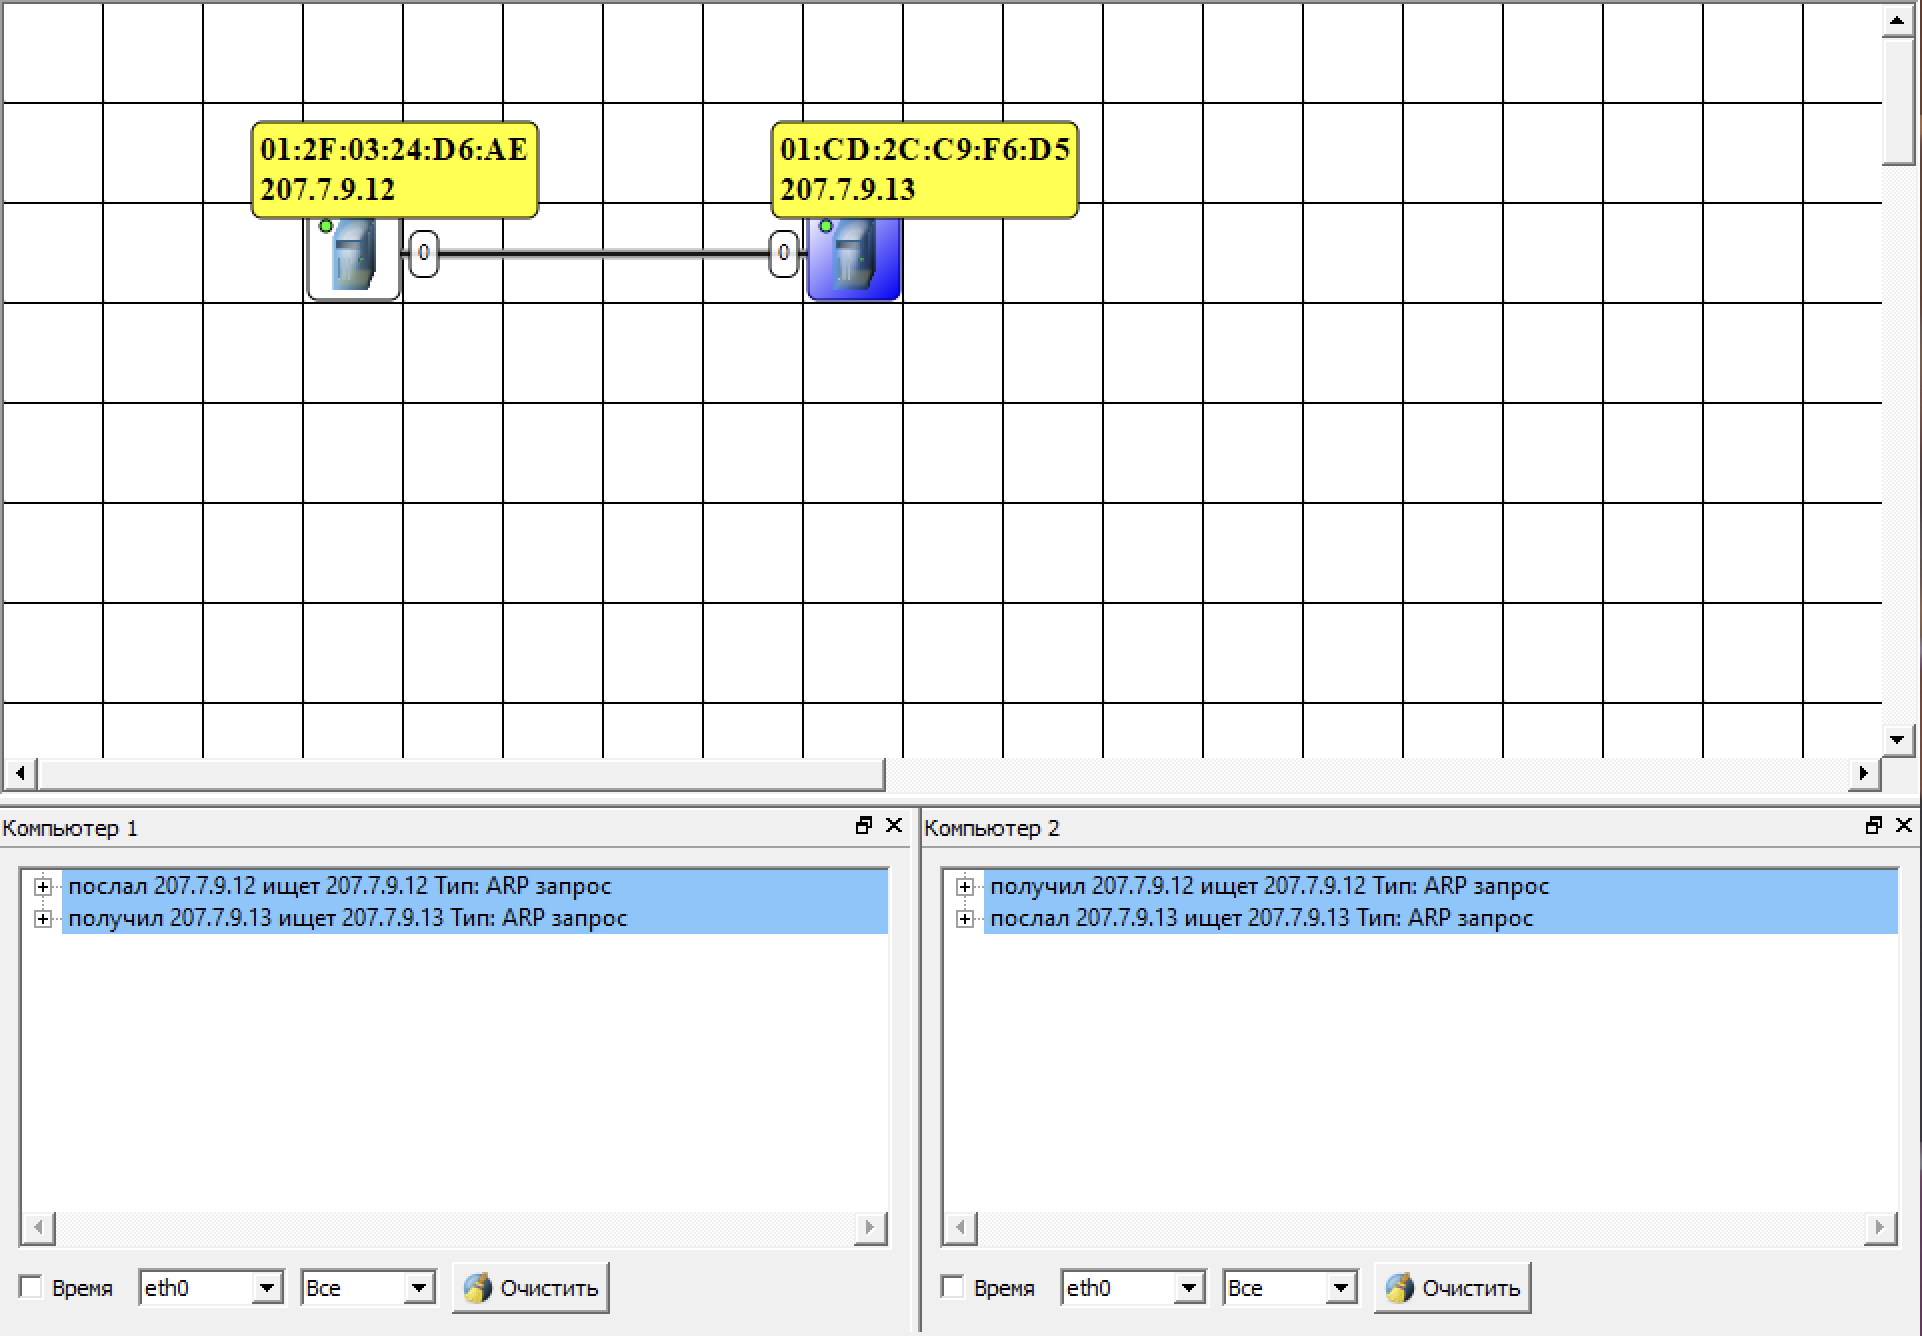
\includegraphics[width=0.8\textwidth]{image/ip-addresses.png}
  \caption{Назначение IP-адресов компьютерам.}
\end{figure}

Настроил интерфейс каждого компьютера (сетевой карты), вручную присвоив ему IP-адрес из заданного набора адресов, маска появилась автоматически.

После присвоения IP-адреса устройству в локальной сети происходит ряд сервисных процессов, в том числе передача различных служебных сообщений для настройки и обмена информацией с другими устройствами в сети.
\subsubsection{ARP-запрос и ARP-ответ}
\begin{figure}[H]
  \centering
  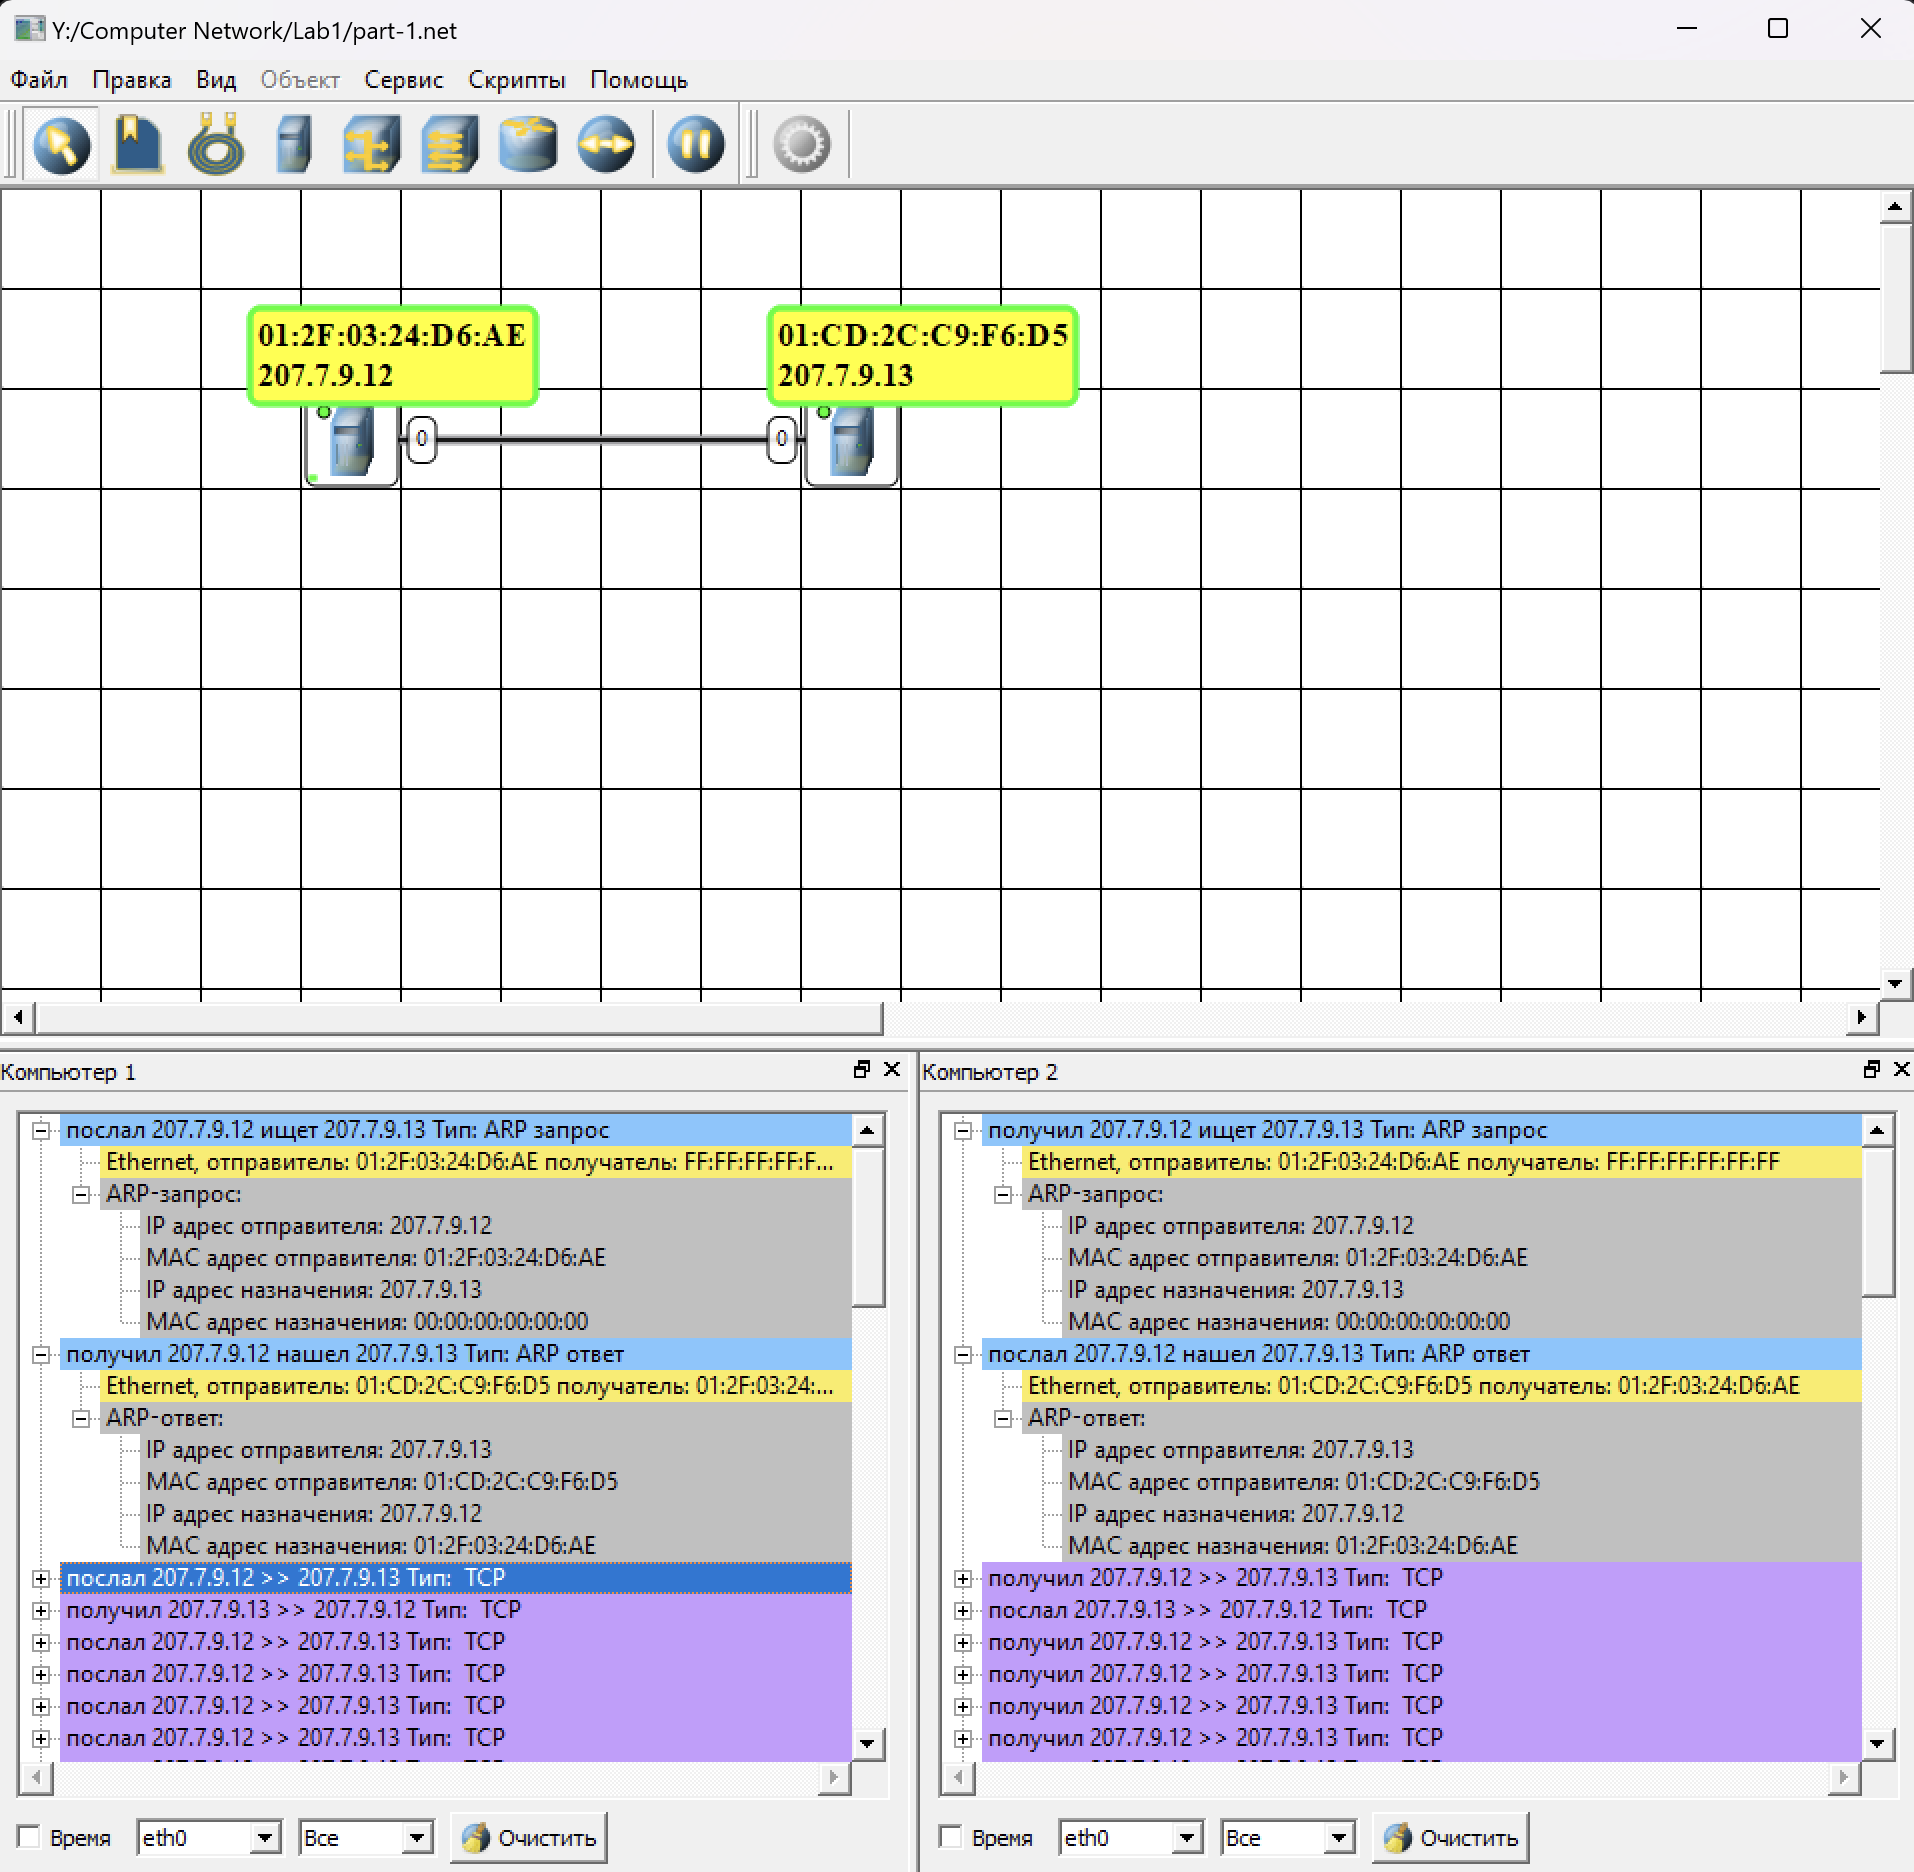
\includegraphics[width=0.8\textwidth]{image/arp-req-resp.png}
  \caption{ARP запрос/ответ.}
\end{figure}
Пакеты передаются по канальной среде, инкапсулированные в кадры. Кадры содержат уникальную идентифицирующую информацию для источника и получателя канальной среды, например MAC-адреса. Устройствам в канальной среде нужен способ определения идентификаторов канальной среды своих соседей, чтобы кадры отправлялись в нужное место назначения. Одним из таких механизмов определения идентификаторов канальной среды является протокол разрешения адресов (ARP).

Устройство, которое хочет найти идентификатор канальной среды другого устройства, создает пакет ARP-запроса. 

Этот запрос включает в себя IP-адрес устройства, для которого нужно найти MAC-адрес,
а также IP-адрес и MAC-адрес устройства, отправляющего запрос.

Пакет ARP-запроса помещается в кадр. MAC-адрес источника тот же, что и у источника, а MAC-адрес назначения - широковещательный адрес (FFFF.FFFF.FFFF).

Один из хостов, которые получили этот широковещательный пакет, видит, что IP-адрес принадлежит ему. И в ответ шлет свой MAC-адрес.
Соответсвующая запись связки IP-адреса и MAC-адреса добавляется в ARP-таблицу.

В дальнейшем, когда устройство хочет отправить пакет другому устройству в локальной сети, оно сначала проверяет ARP-таблицу на наличие соответствующей записи. Если запись есть, то устройство использует MAC-адрес из этой записи для отправки пакета. Если записи нет, то устройство отправляет ARP-запрос, чтобы узнать MAC-адрес устройства.

\begin{figure}[H]
  \centering
  \begin{minipage}[b]{0.49\textwidth}
      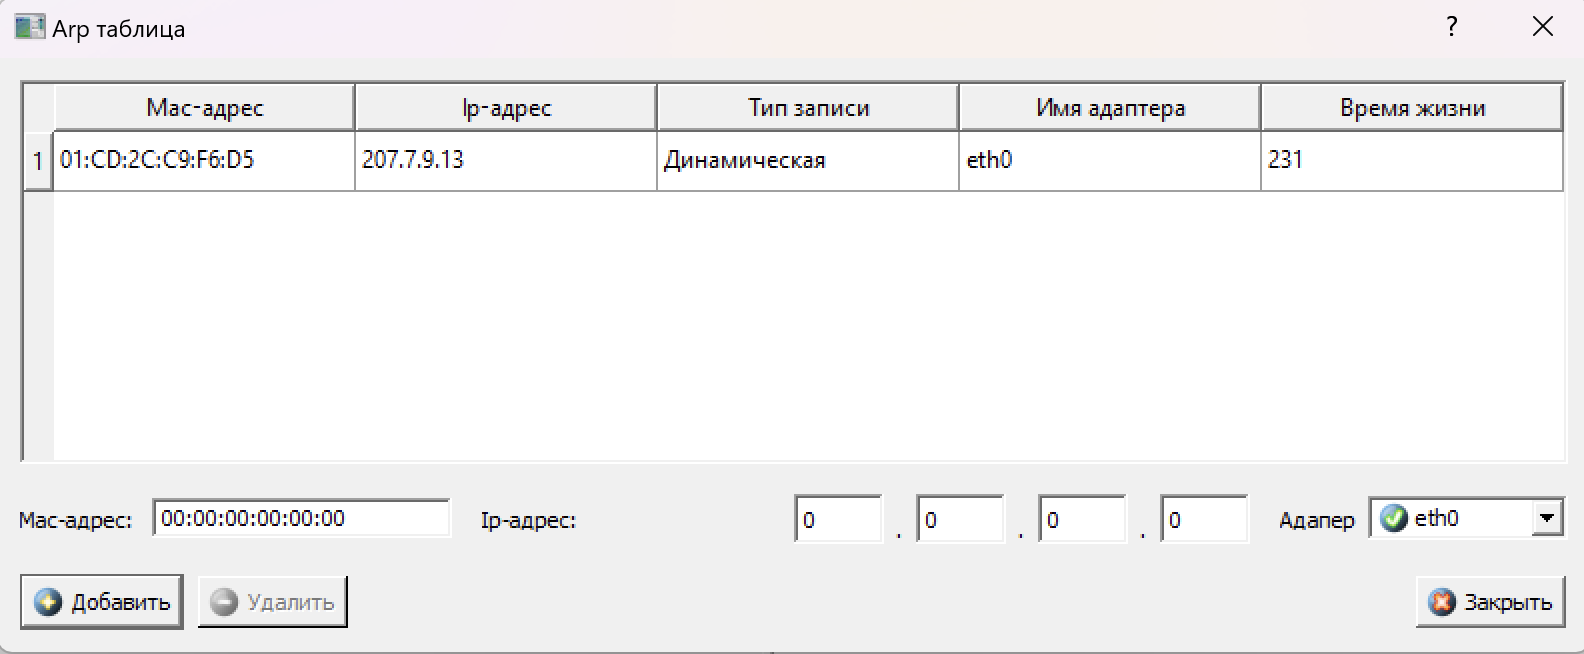
\includegraphics[width=\textwidth]{image/arp-table-1}
      \caption{ARP-таблица компьютера 1.png}
  \end{minipage}
  \hfill
  \begin{minipage}[b]{0.49\textwidth}
      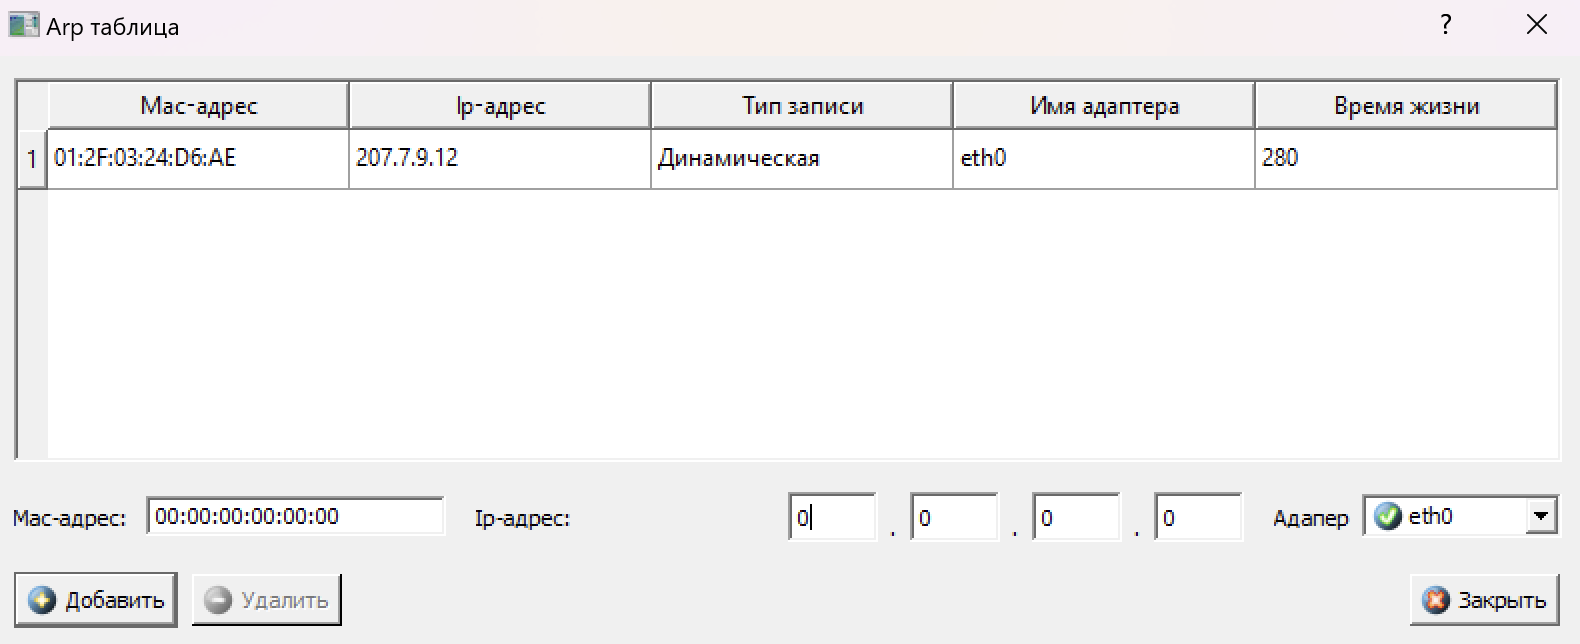
\includegraphics[width=\textwidth]{image/arp-table-2.png}
      \caption{ARP-таблица компьютера 2.}
  \end{minipage}
\end{figure}

\subsection{Анализ таблиц.}
\begin{itemize}
  \item В таблице маршрутизации изменений нет.
  \item В ARP-таблице компьютера 1 появилась запись о MAC-адресе компьютера 2, аналогично в ARP-таблице компьютера 2 появилась запись о MAC-адресе компьютера 1.
\end{itemize}

Содержимое таблиц маршрутизации и ARP-таблицы было описано в пунктах \hyperref[sec:routing]{2.1.1} и \hyperref[sec:arp]{2.1.2} соответственно.
\subsection{Тестирование сети (отправка пакетов).}
\begin{figure}[H]
  \centering
  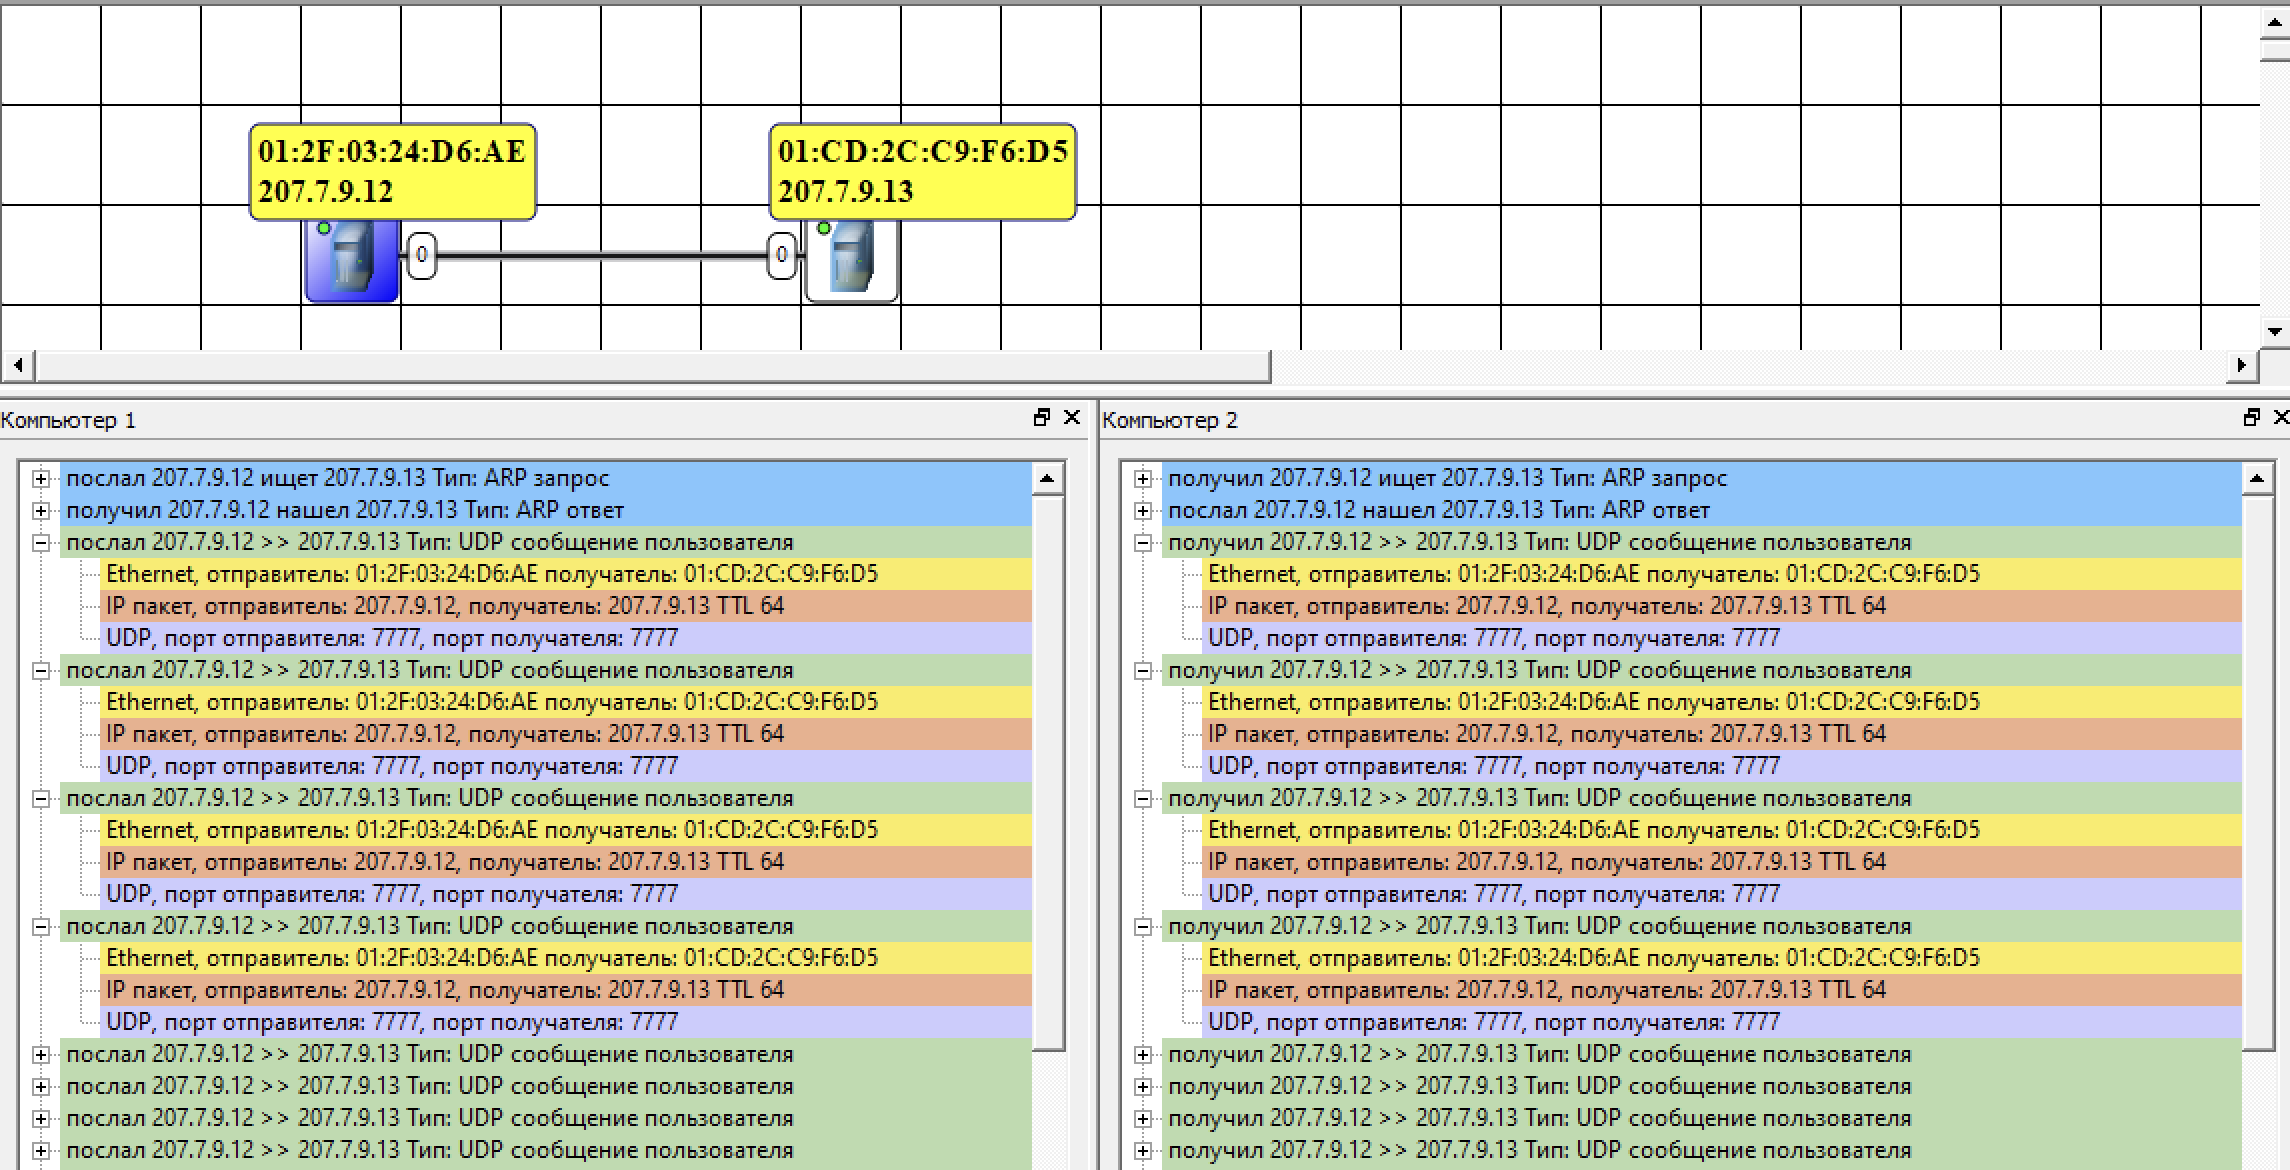
\includegraphics[width=0.8\textwidth]{image/udp.png}
  \caption{Отправка пакетов udp от компьютера 1 к компьютеру 2.}
\end{figure}
\begin{itemize}
  \item {
    \textbf{Какие пакеты и кадры передаются в сети:}
      \begin{itemize}
        \item Пакеты: Данные разделяются на UDP-пакеты. Заголовок UDP содержит информацию о портах отправителя и получателя, длине пакета и контрольной сумме (опционально).
        \item Кадры: UDP-пакеты инкапсулируются в кадры. Кадры содержат MAC-адреса источника и получателя, а также информацию о протоколе передачи данных.
      \end{itemize}
  }
  \item {
    \textbf{В какой последовательности передаются пакеты и кадры:}
    UDP-пакеты могут передаваться в произвольном порядке, без какой-либо гарантии последовательной доставки получателю.
  }
  \item {
    \textbf{Какая информация содержится в пакетах и кадрах}
    \begin{itemize}
      \item Пакеты: данные, заголовок UDP, IP-адреса источника и получателя, время жизни пакета.
      \item Кадры: MAC-адреса источника и получателя, информация о протоколе передачи данных.
    \end{itemize}
  }
  \item {
    \textbf{Появились ли изменения (записи) в таблицах маршрутизации и a таблицах, и если «да», то, когда и как формируются записи?}
      
      Изменения в таблицах маршрутизации и ARP-таблицах могли появиться, если:
      \begin{enumerate}
        \item Устройство получает новую информацию о соответствии IP-адресов и MAC-адресов других устройств в сети, тогда в ARP-таблице появляется новая запись.
        \item Маршрутизатор принимает новый маршрут для передачи пакетов, тогда в таблице маршрутизации появляется новая запись.
      \end{enumerate}
  }
\section{Линейная сеть из трех компьютеров}
\subsection{Построение сети с тремя компьютерами и анализ таблиц.}
\begin{figure}[H]
  \centering
  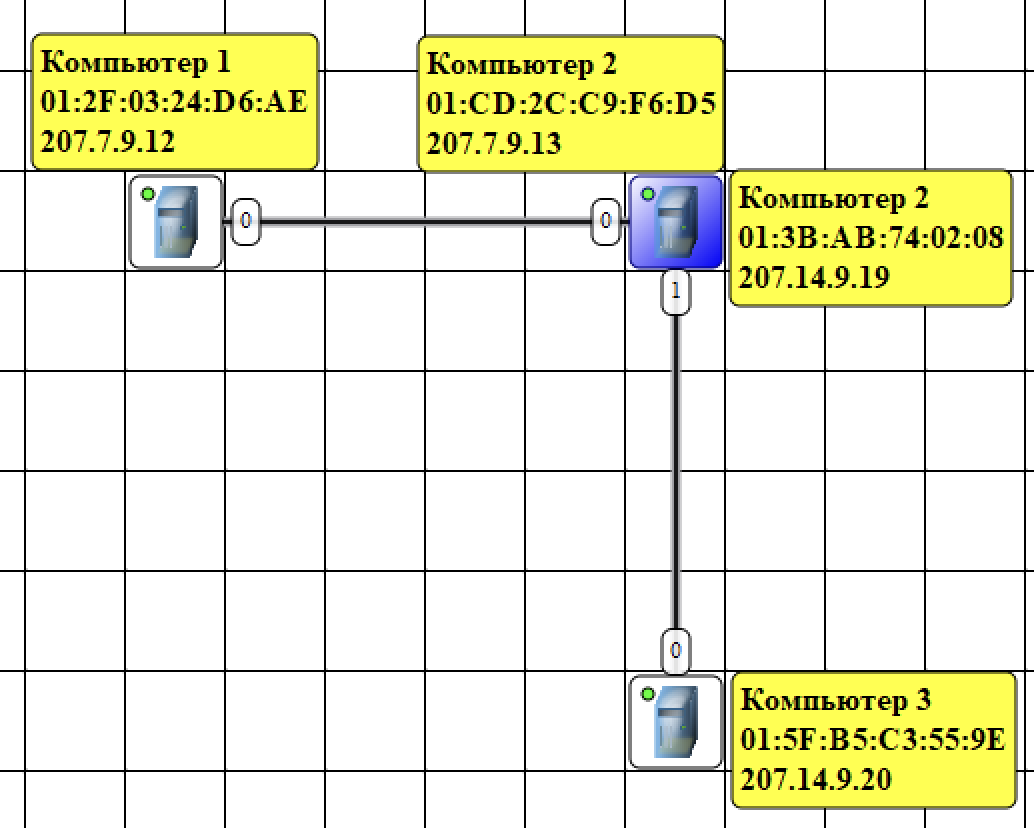
\includegraphics[width=0.8\textwidth]{image/3-computers.png}
\end{figure}
Сделал сеть из 3х компьютеров, назначил им имена и IP-адреса.
Добавили в Компьютер 2 дополнительный интерфейс и настроили шлюзы всех компьютеров.
\begin{figure}[H]
  \centering
  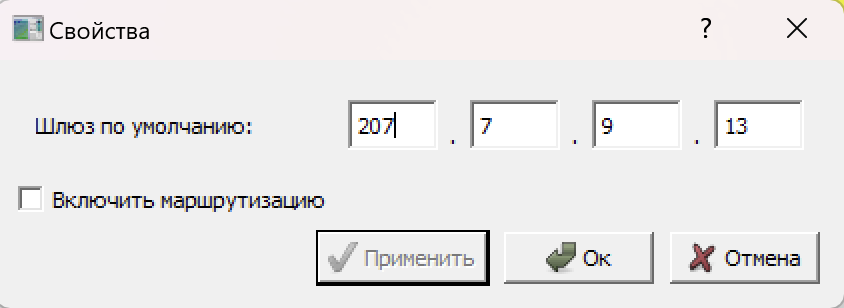
\includegraphics[width=0.8\textwidth]{image/gate-1.png}
  \caption{Настройка шлюзов Компьютера 1.}
\end{figure}
\begin{figure}[H]
  \centering
  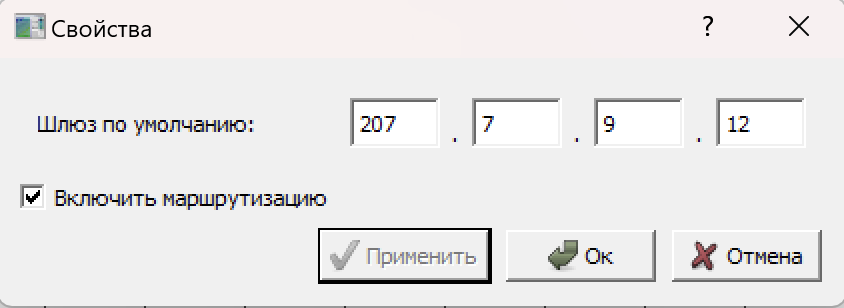
\includegraphics[width=0.8\textwidth]{image/gate-2.png}
  \caption{Настройка шлюзов Компьютера 2.}
\end{figure}
\begin{figure}[H]
  \centering
  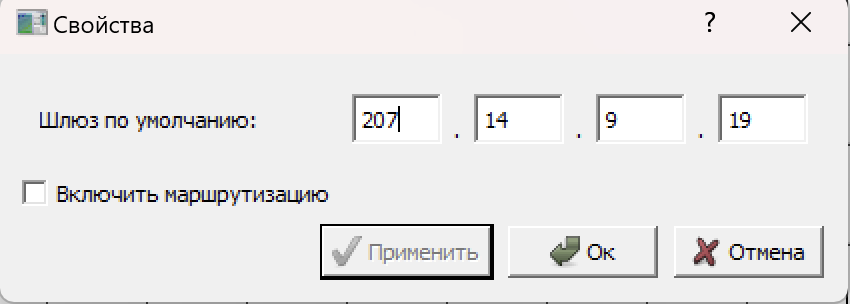
\includegraphics[width=0.8\textwidth]{image/gate-3.png}
  \caption{Настройка шлюзов Компьютера 3.}
\end{figure}
\subsubsection{Таблицы маршрутизации}
\begin{figure}[H]
  \centering
  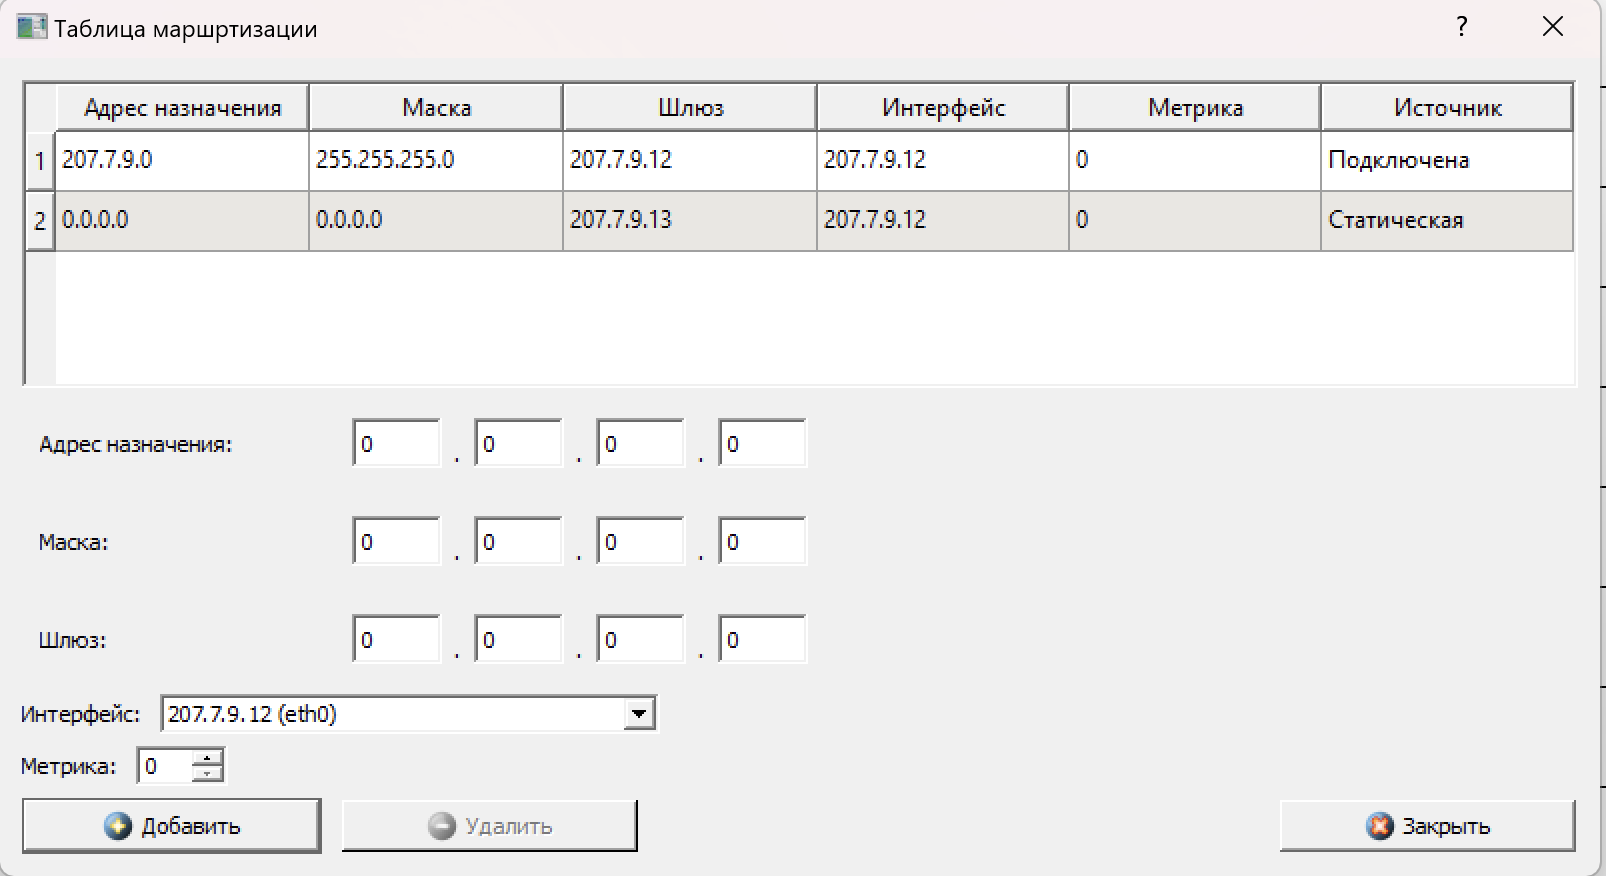
\includegraphics[width=0.8\textwidth]{image/routing-table-1.png}
  \caption{Таблица маршрутизации Компьютера 1.}
\end{figure}
\begin{figure}[H]
  \centering
  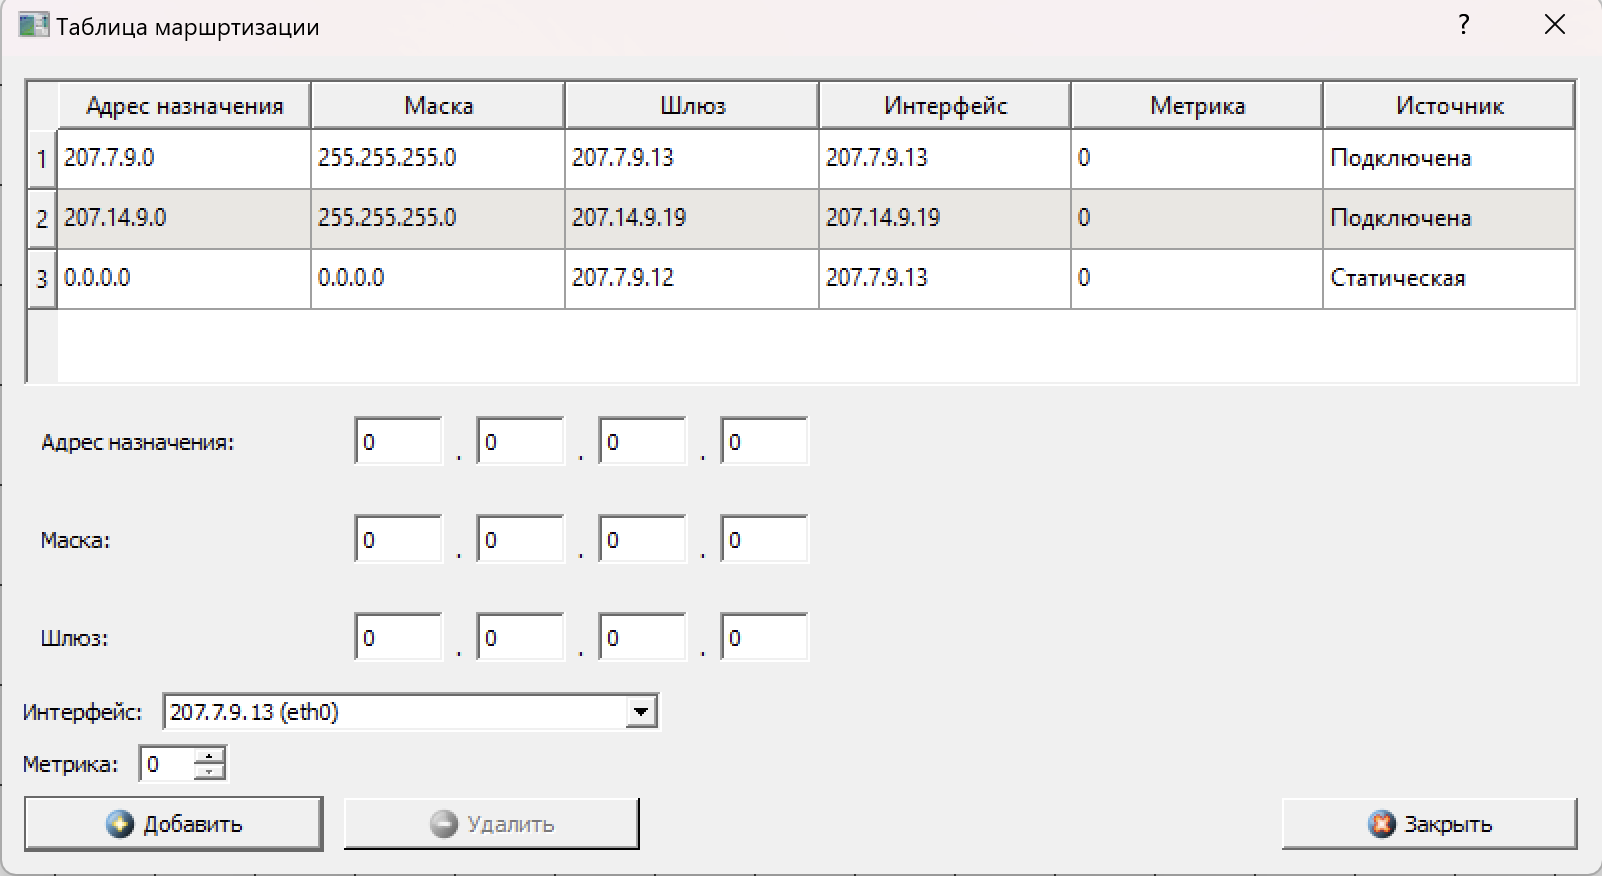
\includegraphics[width=0.8\textwidth]{image/routing-table-2-2.png}
  \caption{Таблица маршрутизации Компьютера 2.}
\end{figure}
\begin{figure}[H]
  \centering
  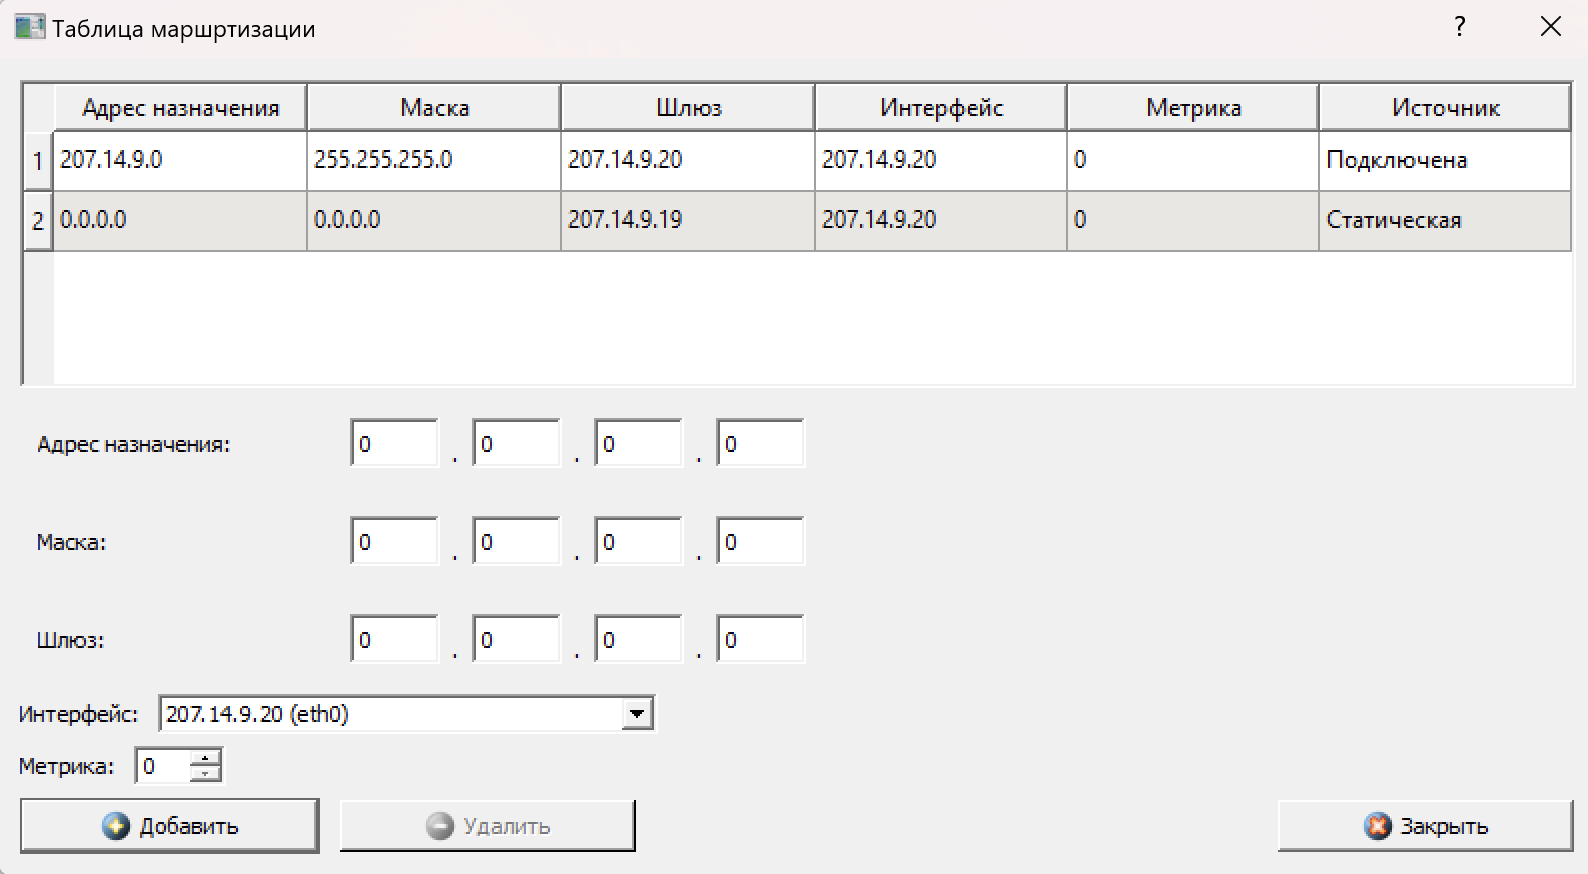
\includegraphics[width=0.8\textwidth]{image/routing-table-3.png}
  \caption{Таблица маршрутизации Компьютера 3.}
\end{figure}

Кроме стандартных записей, что адреса внутри данной сети могут быть достигнуты непосредственно. 
Добавились статические маршруты с адрессом и маской 0.0.0.0, они говорят, что все остальные адреса могут быть достигнуты через шлюз указанный в столбце "шлюз".

Статические маршруты - это записи, сделанные в таблице маршрутизации неавтоматическим способом и являющиеся фиксированными, а не результатом работы протоколов маршрутизации, адаптированных к изменяющимся условиям сети.

Компьютер 2 имеет 2 сетевых интерфейса и 2 шлюза, что позволяет ему быть маршрутизатором между двумя сетями.
Но в случае, если адрес назначения не принадлежит ни одной из сетей, пакеты будут отправляться на шлюз первой сети.

\subsection{Тестирование сети (отправка пакетов)}
\begin{figure}[H]
  \centering
  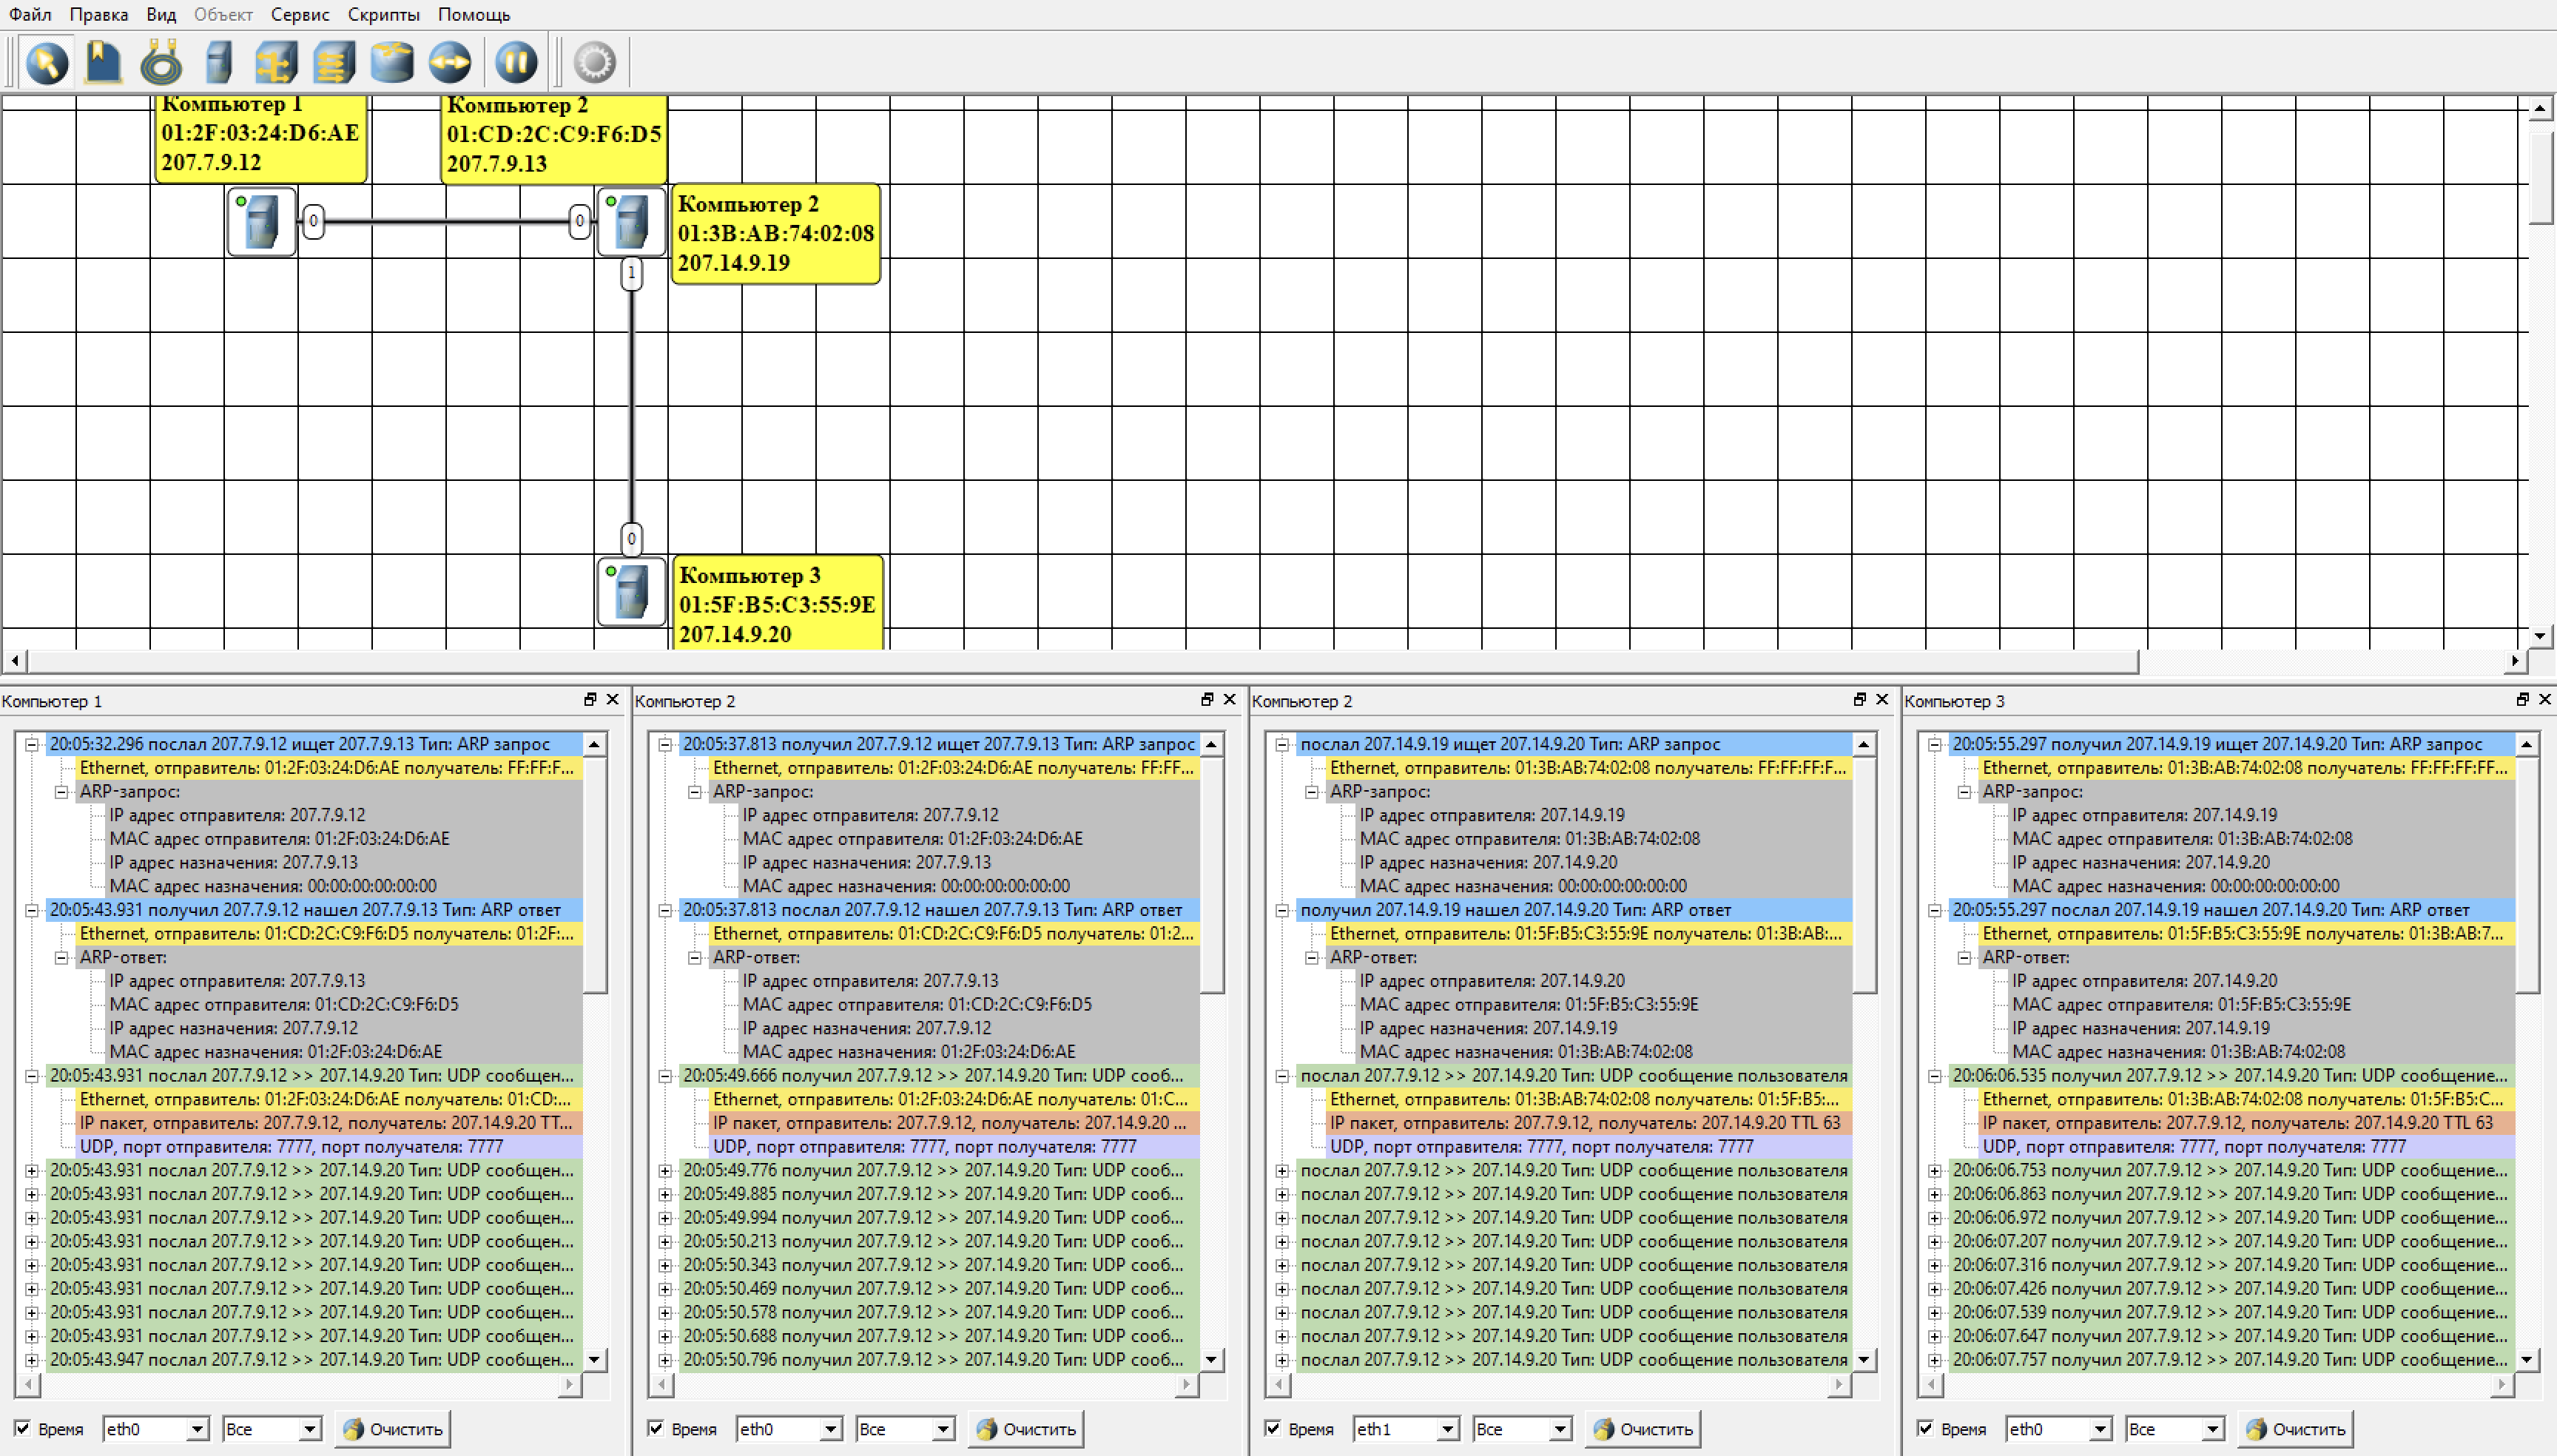
\includegraphics[width=0.8\textwidth]{image/udp-linear-topo.png}
  \caption{Отправка пакетов udp от компьютера 1 к компьютеру 3.}
\end{figure}

Видим, что как и согласно таблице маршрутизации, компьютер 1 получая задачу отправить пакет на адрес незнакомой сети пользуется правилом 0.0.0.0 и отправляет ARP-запрос на поиск MAC-адреса компьютера 2. После получения ответа, пакеты отправляются на компьютер 2.
Далее, что тоже отражено в таблице маршрутизации, компьютер 2 видя, что адрес сети назначения принадлежит сети 2, перенаправляет пакеты на свой второй сетевой интерфейс. Второй сетевой интерфейс отправляет ARP-запрос на поиск MAC-адреса компьютера 3 и после получения ответа отправляет пакеты на компьютер 3.
\end{itemize}

\section{Полносвязная сеть из трех компьютеров}
\subsection{Формирование полносвязной компьютерной сети.}
Сделал полносвязную сеть из 3х компьютеров, назначил им имена и IP-адреса.
Каждый компьютер имеет 2 сетевых интерфейса.
Каждому компьютеру назначил шлюз по умолчанию.
\begin{figure}[H]
  \centering
  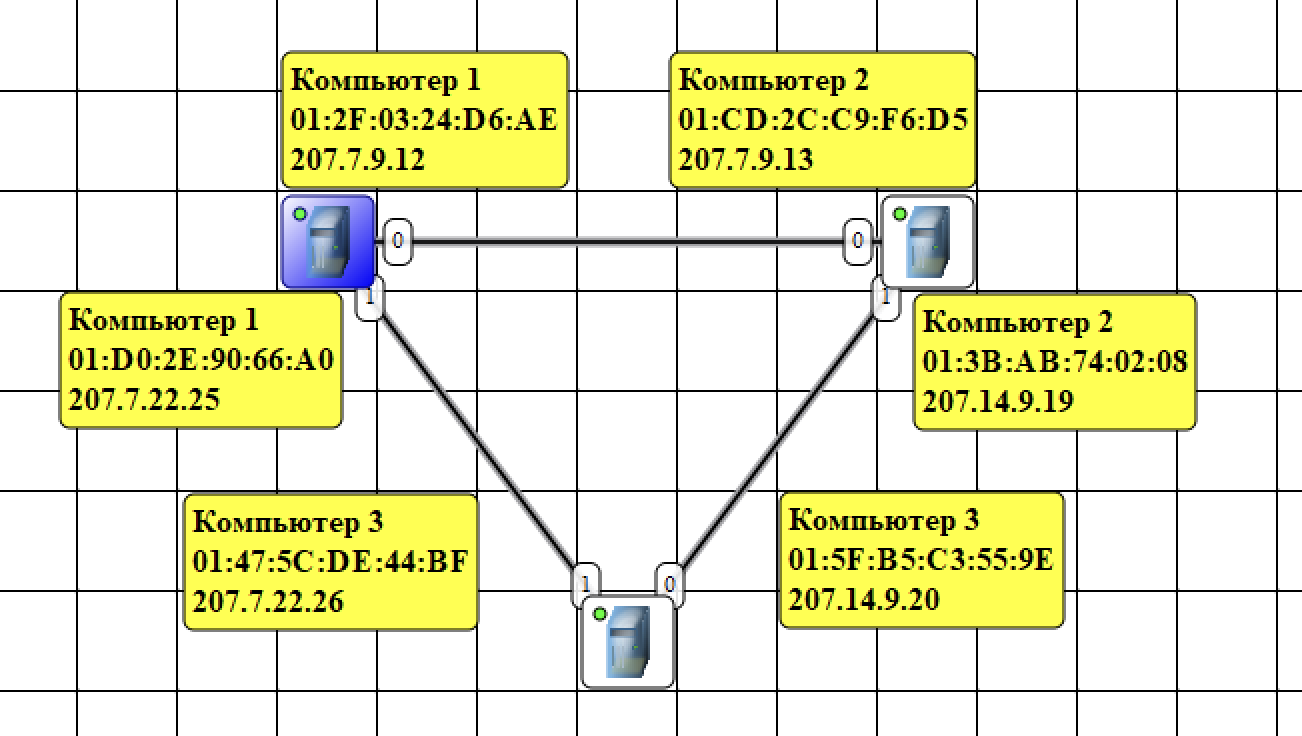
\includegraphics[width=0.8\textwidth]{image/part3/topology.png}
  \caption{Полносвязная сеть из 3х компьютеров.}
\end{figure}

\begin{figure}[H]
  \centering
  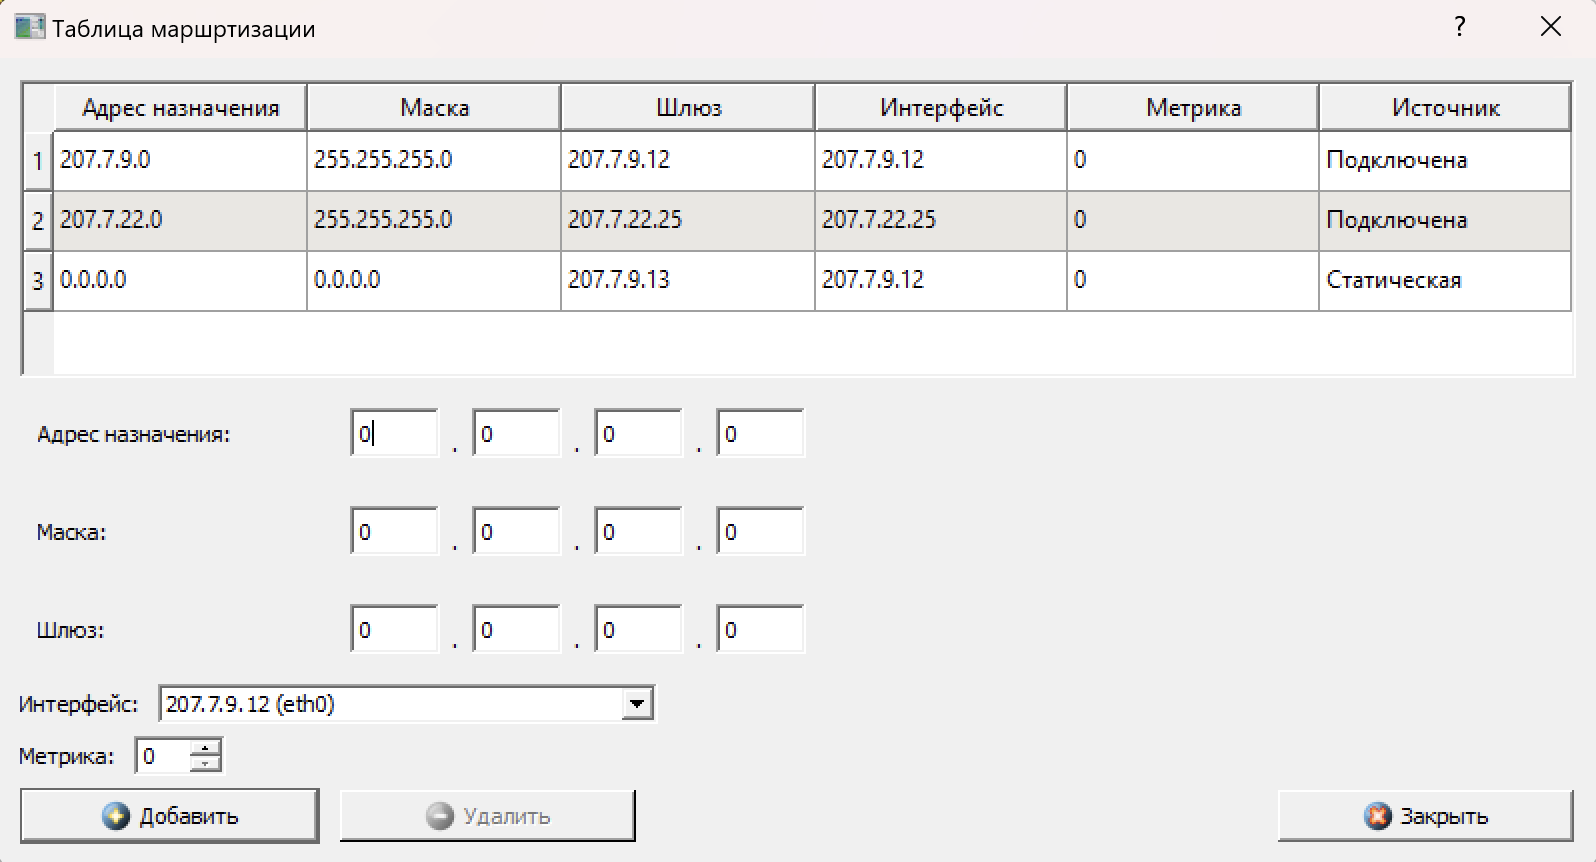
\includegraphics[width=0.8\textwidth]{image/part3/routing-table-1.png}
  \caption{Таблица маршрутизации Компьютера 1.}
\end{figure}
Шлюз по умолчанию -- Компьютер 2
\begin{figure}[H]
  \centering
  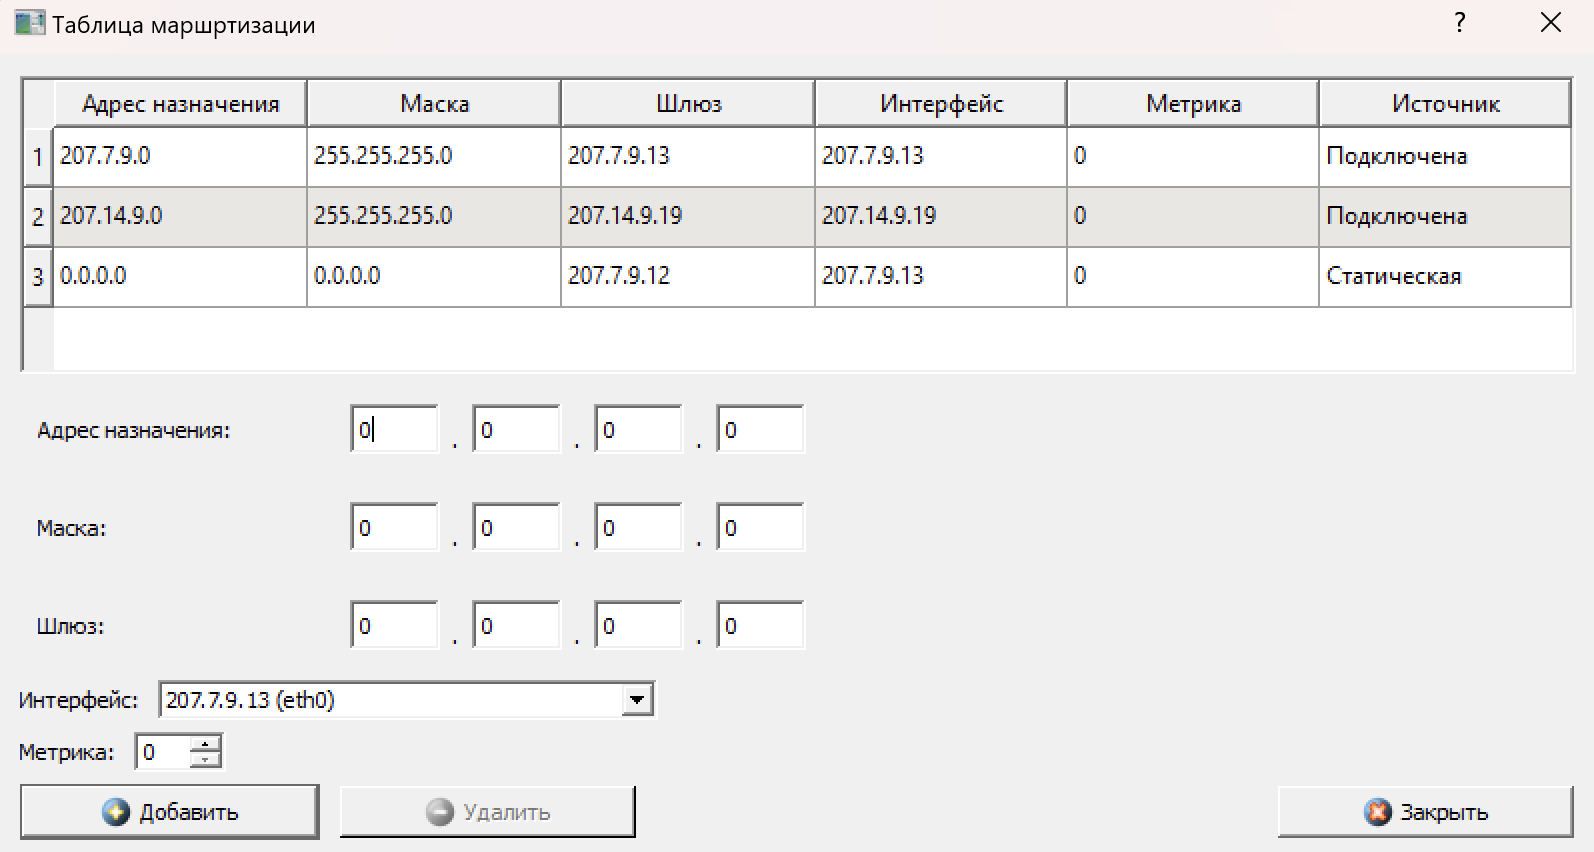
\includegraphics[width=0.8\textwidth]{image/part3/routing-table-2.png}
  \caption{Таблица маршрутизации Компьютера 2.}
\end{figure}
Шлюз по умолчанию -- Компьютер 2
\begin{figure}[H]
  \centering
  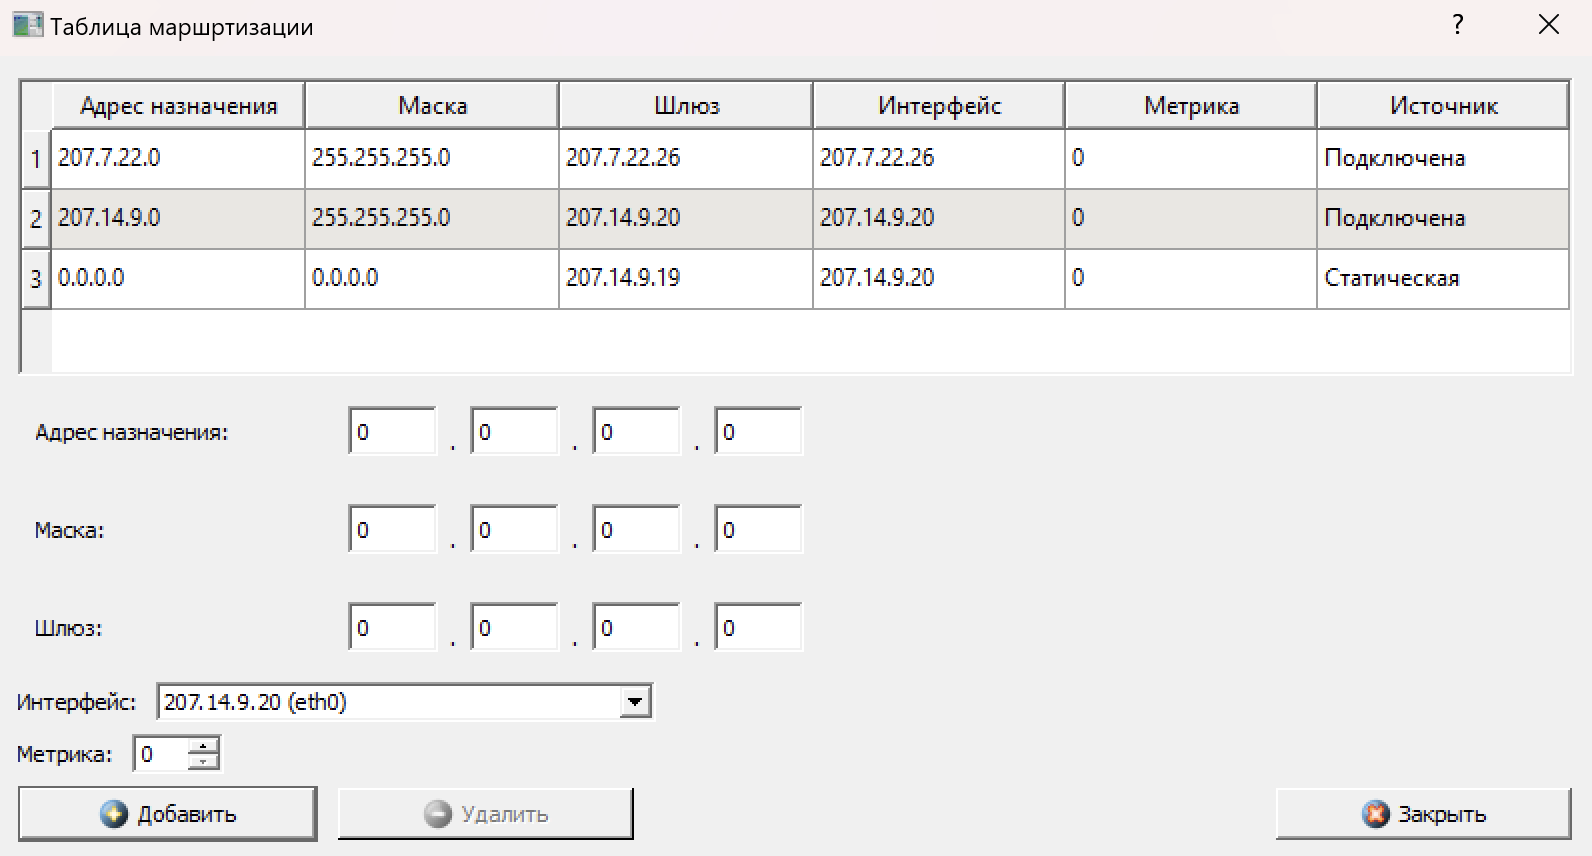
\includegraphics[width=0.8\textwidth]{image/part3/routing-table-3.png}
  \caption{Таблица маршрутизации Компьютера 3.}
\end{figure}
Шлюз по умолчанию -- Компьютер 2
\subsection{Тестирование сети (отправка пакетов).}
\subsubsection{Случай 1}
\begin{figure}[H]
  \centering
  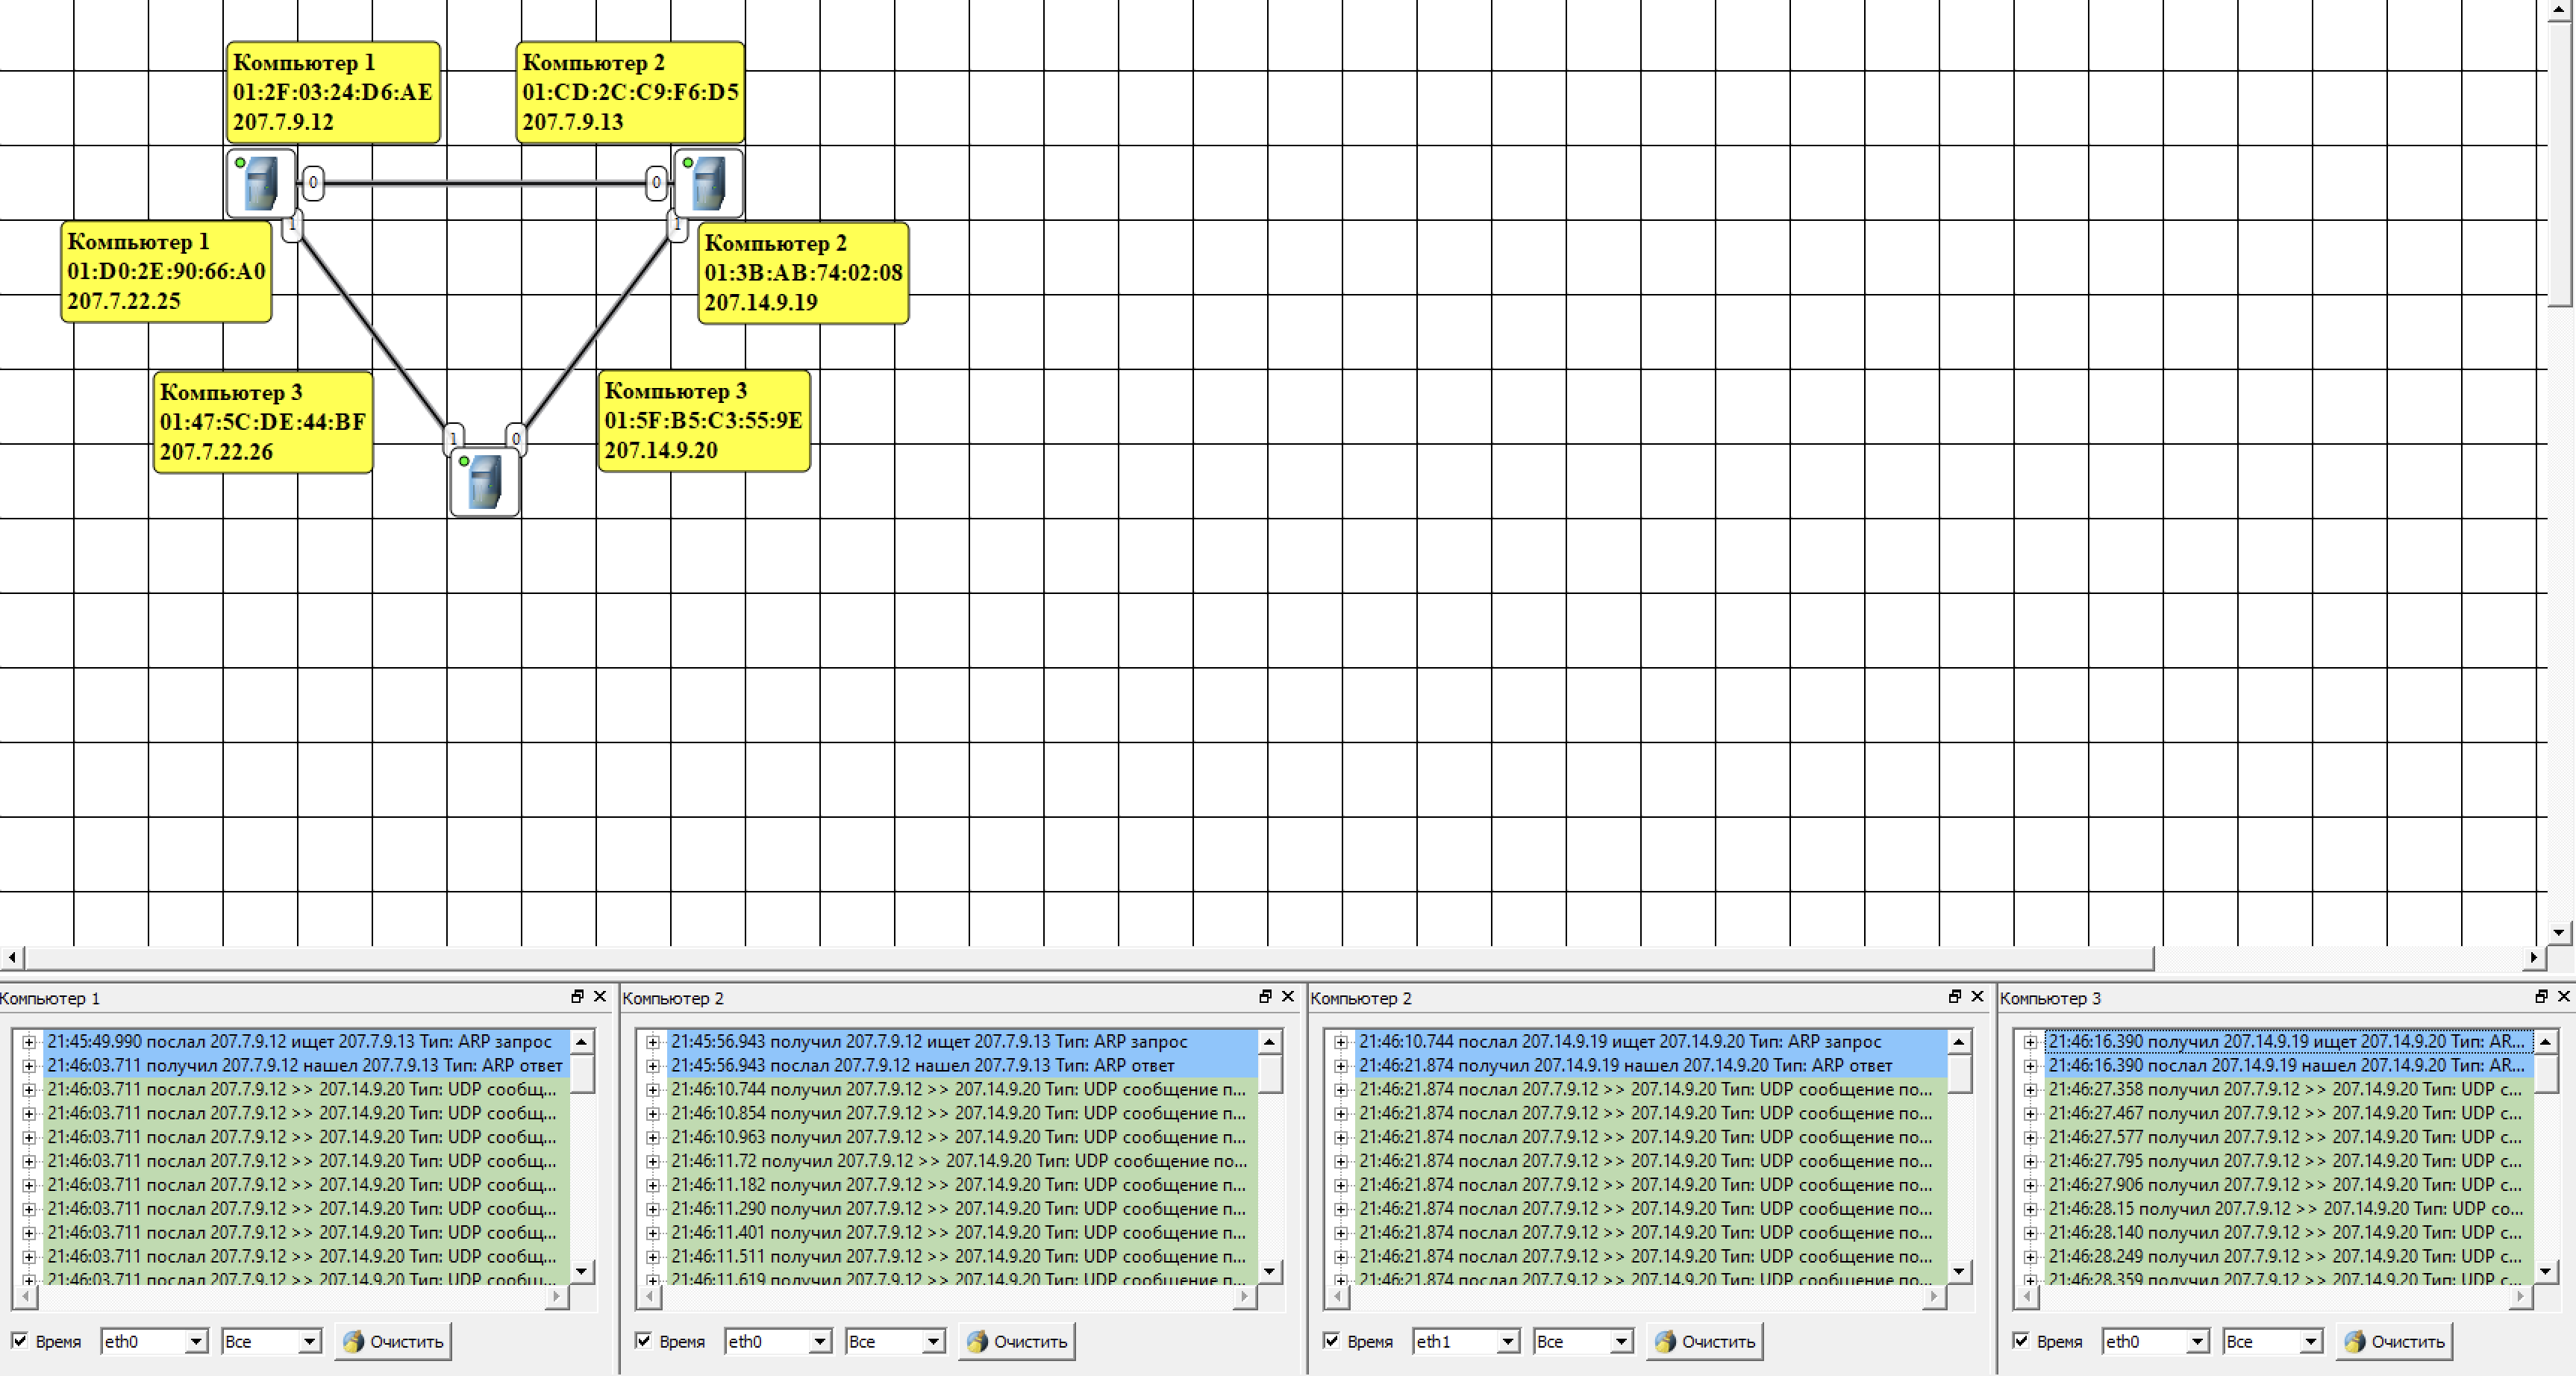
\includegraphics[width=0.8\textwidth]{image/part3/udp-1.png}
  \caption{Отправка пакетов udp от компьютера 1 к компьютеру 3 на интерфейс 0.}
\end{figure}
Мы видим, что в данном случае пакеты отправляются как и в случае с линейной топологией. Пакеты отправляются на шлюз по умолчанию, который в данном случае является Компьютер 2. Компьютер 2, видя что адрес назначения принадлежит сети 2, перенаправляет пакеты на свой второй сетевой интерфейс. Второй сетевой интерфейс отправляет ARP-запрос на поиск MAC-адреса компьютера 3 и после получения ответа отправляет пакеты на компьютер 3.
\subsubsection{Изменение ARP-таблиц после отправки пакетов в случае 1}
\begin{figure}[H]
  \centering
  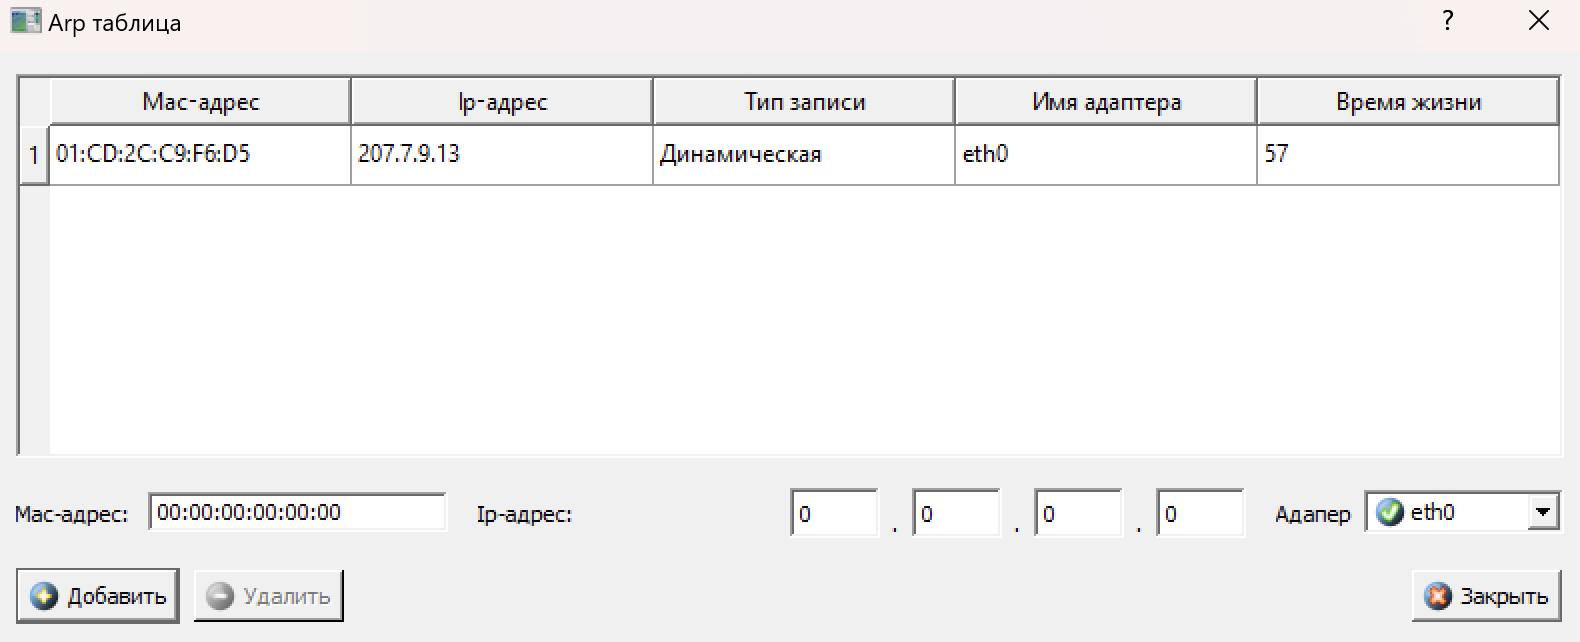
\includegraphics[width=0.8\textwidth]{image/part3/arp-1-1.png}
  \caption{ARP-таблица Компьютера 1 после отправки пакетов в случае 1.}
\end{figure}
\begin{figure}[H]
  \centering
  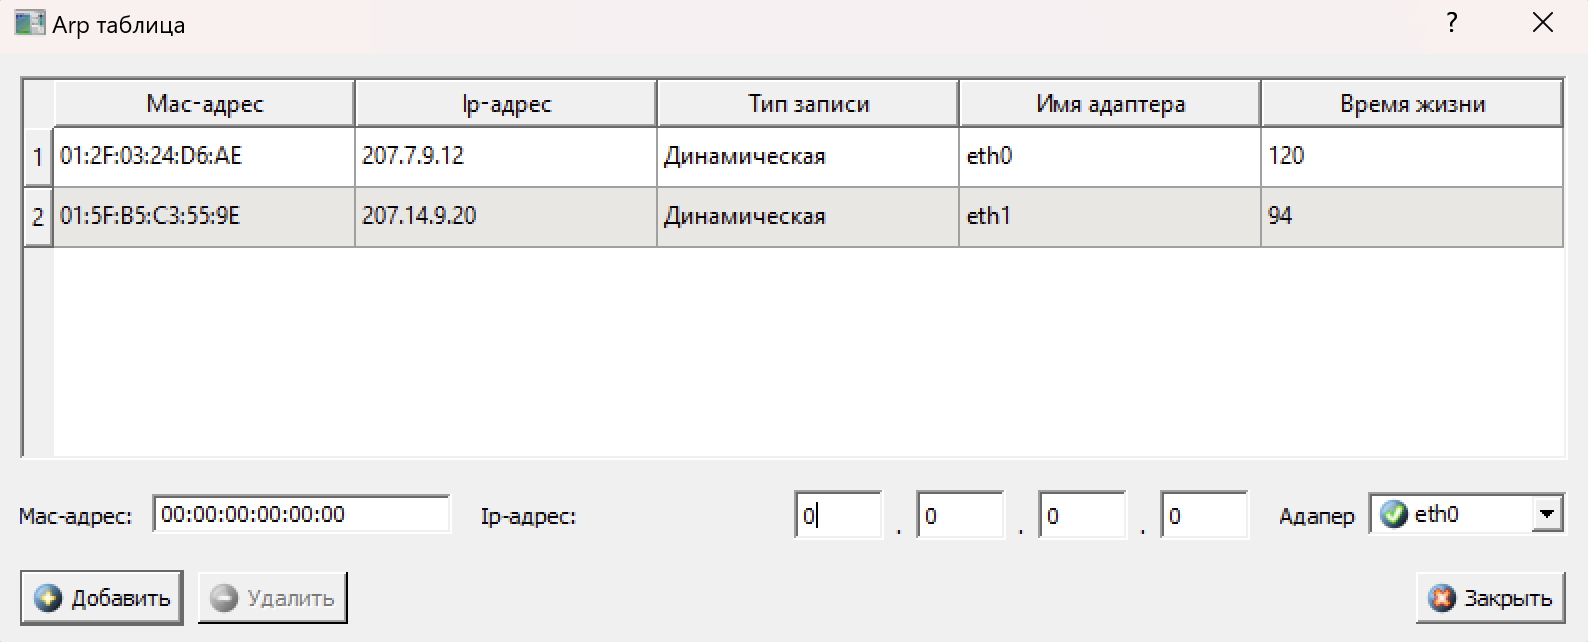
\includegraphics[width=0.8\textwidth]{image/part3/arp-1-2.png}
  \caption{ARP-таблица Компьютера 2 после отправки пакетов в случае 1.}
\end{figure}
\begin{figure}[H]
  \centering
  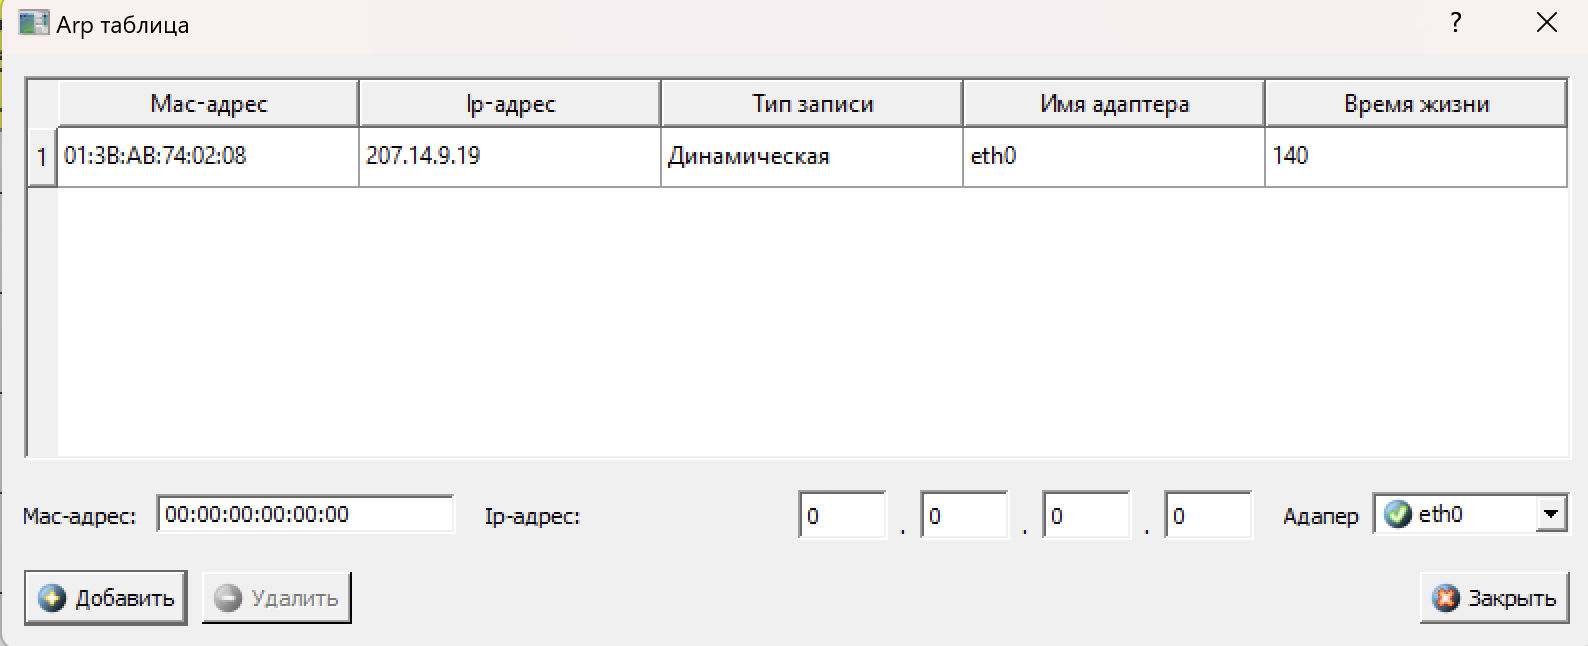
\includegraphics[width=0.8\textwidth]{image/part3/arp-1-3.png}
  \caption{ARP-таблица Компьютера 3 после отправки пакетов в случае 1.}
\end{figure}
\subsubsection{Случай 2}
\begin{figure}[H]
  \centering
  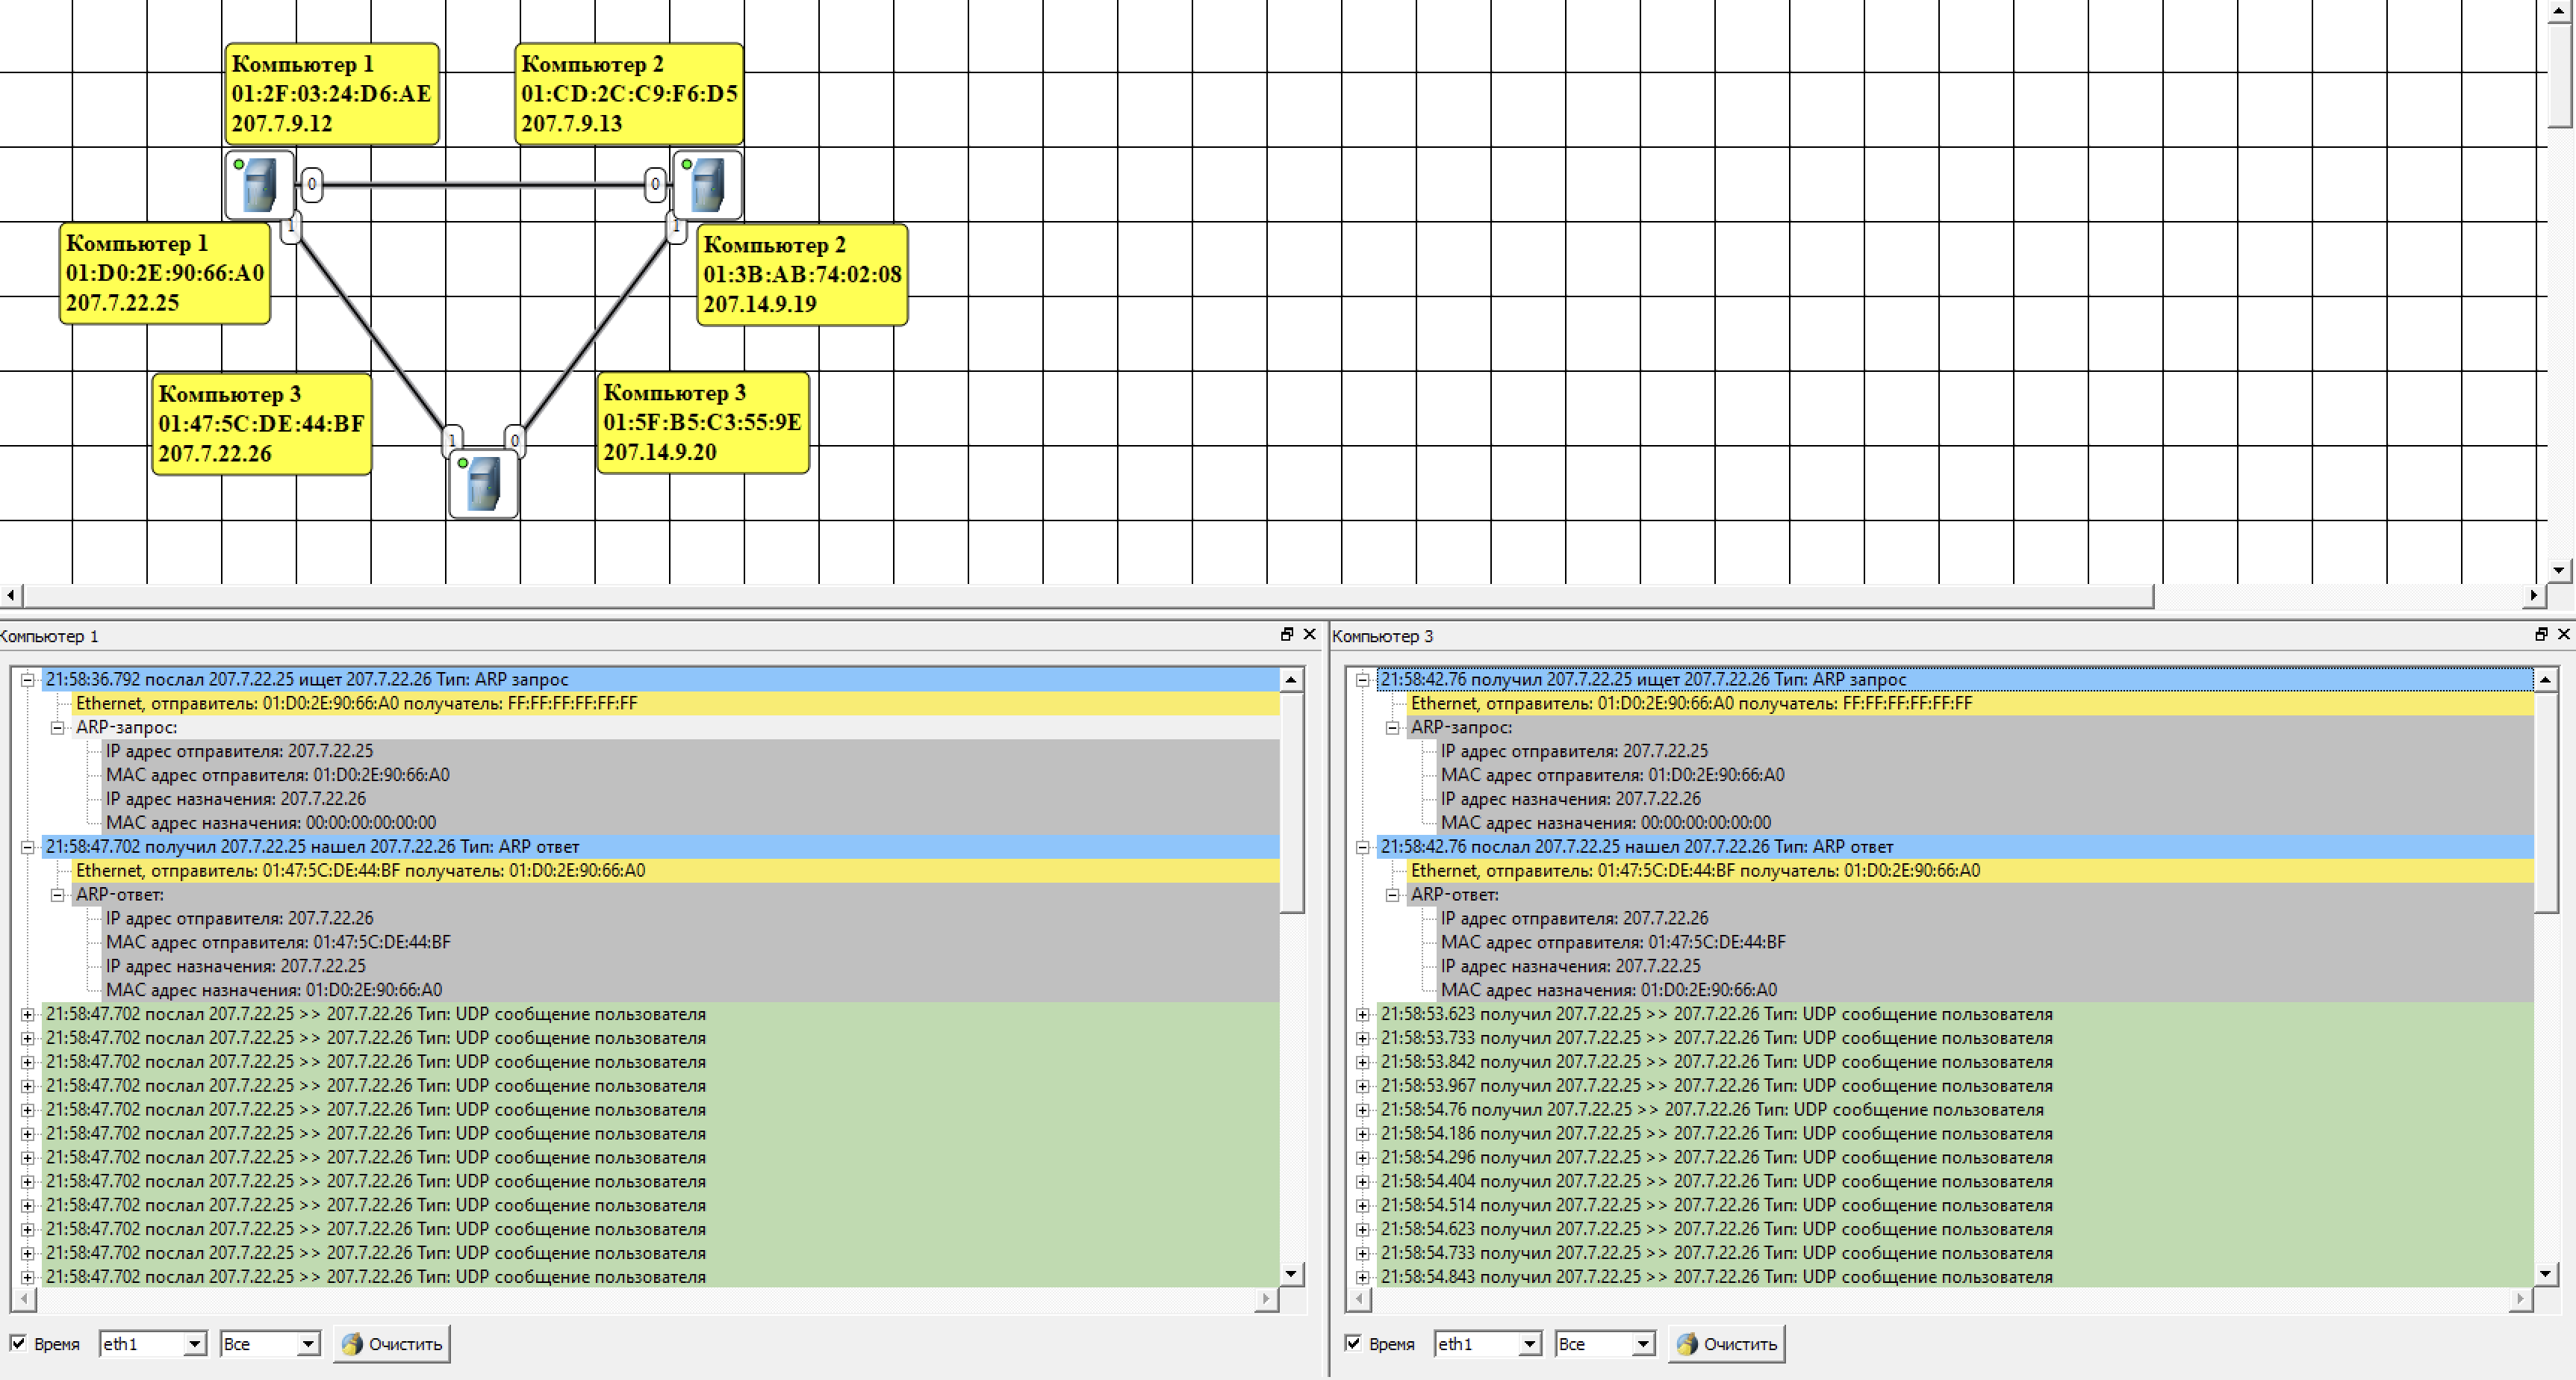
\includegraphics[width=0.8\textwidth]{image/part3/udp-2.png}
  \caption{Отправка пакетов udp от компьютера 1 к компьютеру 3 на интерфейс 1.}
\end{figure}
В данном случае пакеты отправляются напрямую с Компьютера 1 на Компьютер 3.
\subsubsection{Изменение ARP-таблиц после отправки пакетов в случае 2}
\begin{figure}[H]
  \centering
  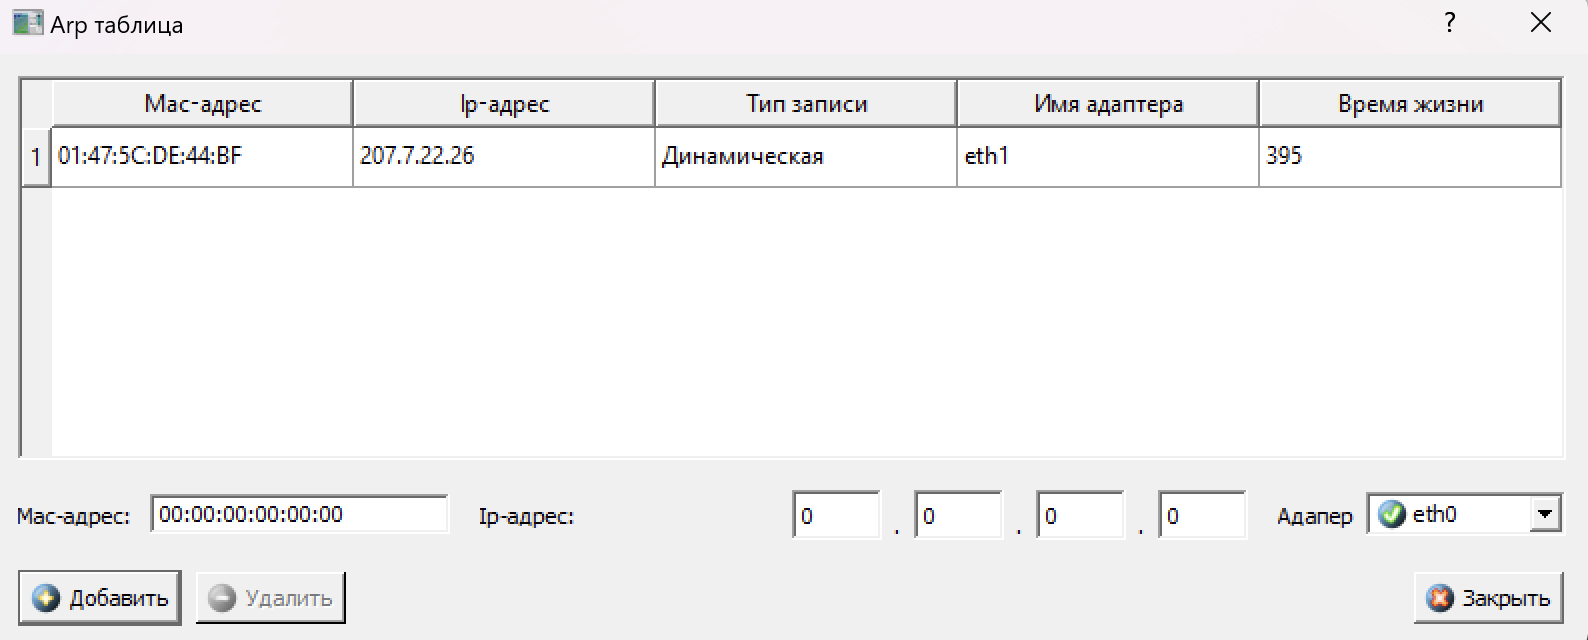
\includegraphics[width=0.8\textwidth]{image/part3/arp-2-1.png}
  \caption{ARP-таблица Компьютера 1 после отправки пакетов в случае 2.}
\end{figure}
Видим, что он MAC-адрес Компьютера 3.
\begin{figure}[H]
  \centering
  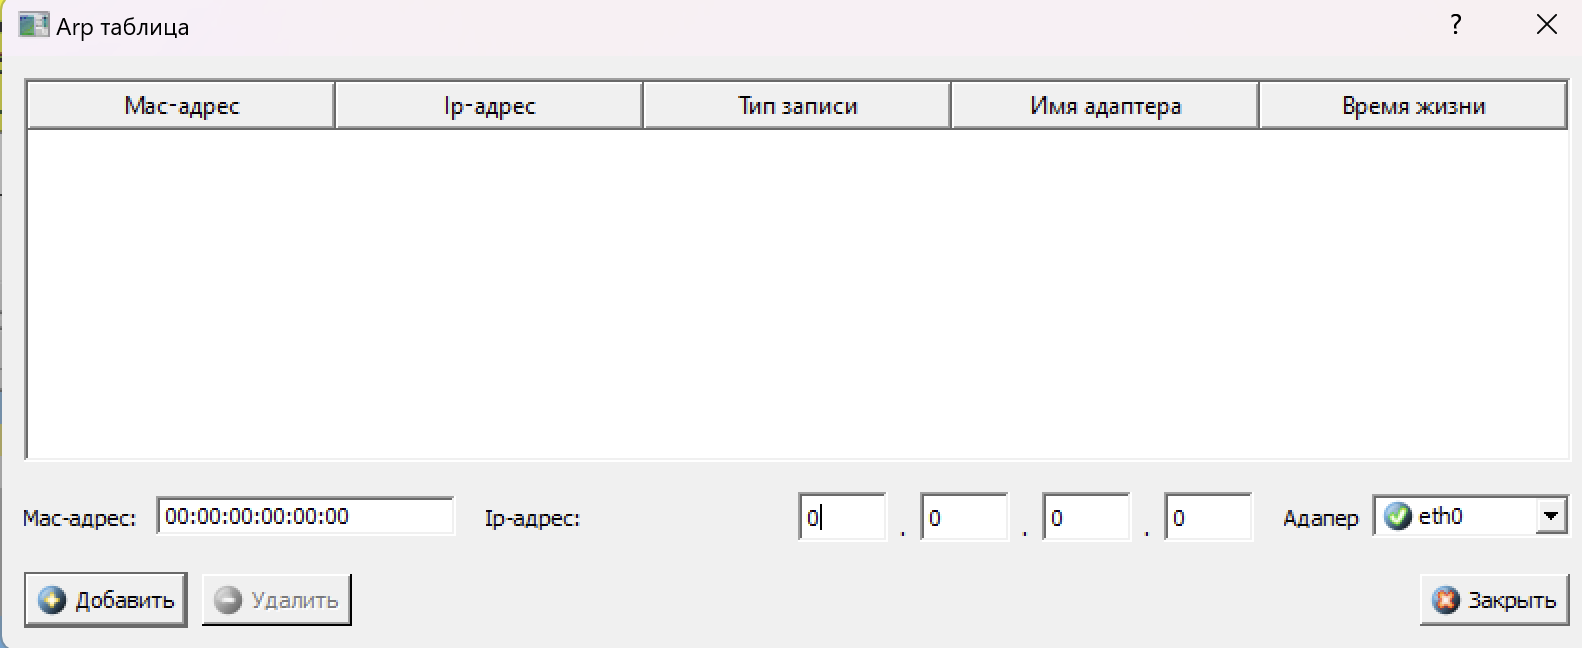
\includegraphics[width=0.8\textwidth]{image/part3/arp-2-2.png}
  \caption{ARP-таблица Компьютера 2 после отправки пакетов в случае 2.}
\end{figure}
ARP-таблица Компьютера 2 как и предполагалось пуста.
\begin{figure}[H]
  \centering
  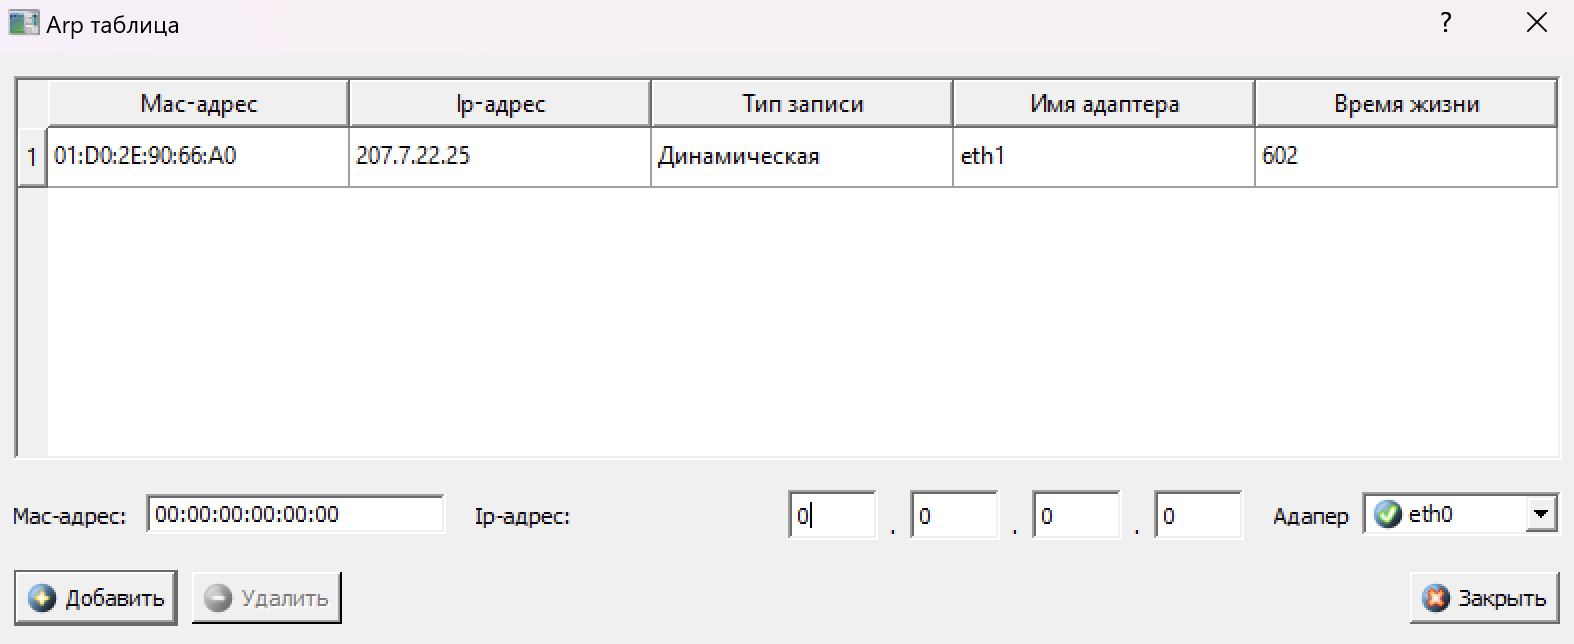
\includegraphics[width=0.8\textwidth]{image/part3/arp-2-3.png}
  \caption{ARP-таблица Компьютера 3 после отправки пакетов в случае 2.}
\end{figure}
Видим, что он MAC-адрес Компьютера 1.
\section{Вывод}
В ходе выполнения лабораторной работы были изучены принципы построения и настройки моделей компьютерных сетей в среде NetEmul. Были построены три простейшие модели компьютерной сети (2 компьютера, линейная сеть из трех компьютеров и полносвязная сеть из трех компьютеров), выполнена настройка сети, заключающаяся в присвоении IP-адрес интерфейсам сети, выполнено тестирование разработанных сетей путем проведения экспериментов по передаче данных на основе протокола UDP. Были сохранены разработанные модели компьютерных сетей для демонстрации процессов передачи данных при защите лабораторной работы.



\end{document}